\chapter[Order theory][Order theory]{Order Theory}\label{app:order-theory}

In this appendix we give an overview of the order theory necessary to study fixed-points of monotone maps.


\section{Objects: Partial orders and lattices}

We begin by recalling the definitions and basic properties of various kinds of ordered sets.

\subsection{Ordered sets}

\makeatletter
\def\dualord{\@ifstar\@dualord\@@dualord}
\def\@dualord#1{(#1)^{\mathit{op}}}
\def\@@dualord#1{#1^{\mathit{op}}}
\makeatother



\makeatletter
\def\upset{\@ifstar\@upset\@@upset}
\def\@upset#1{(#1)^\uparrow}
\def\@@upset#1{#1^\uparrow}
\makeatother



\newcommand{\downset}[1]{#1^\downarrow}

\begin{definition}[Orders]
    A binary relation $\leq$ on a set $P$ is called a \keyword{preorder}\index[subject]{preorder}\index[subject]{preordered set} if $\leq$ is
    %
    \begin{enumdefinition}
        \item reflexive, $x \leq x$ for all $x \in P$, and
        \item transitive, $x \leq y$ and $y \leq z$ implies $x \leq z$ for all $x,y,z \in P$.
    \end{enumdefinition}
    %
    If furthermore $\leq$ is
    %
    \begin{enumdefinition}[resume]
        \item antisymmetric, $x \leq y$ and $y \leq x$ implies $x = y$ for all $x,y \in P$,
    \end{enumdefinition}
    %
    then $\leq$ is called a \keyword{partial order}\index[subject]{partial order}\index[subject]{partially ordered set|see{poset}}, and the pair $(P,\leq)$ is also called a \keyword{poset}\index[subject]{poset}. If $\leq$ is also
    %
    \begin{enumdefinition}[resume]
        \item strongly connected, $x \leq y$ or $y \leq x$ for all $x,y \in P$,
    \end{enumdefinition}
    %
    then $\leq$ is a \keyword{total order}\index[subject]{total order}\index[subject]{totally ordered set}.
\end{definition}
%
Notice that any subset of a preordered set is also preordered with the inherited order. As usual we intentionally conflate a preordered set $(P,\leq)$ and the underlying set $P$ when this does not lead to confusion. We define the \keyword{dual order}\index[subject]{dual order} $\dualord{\leq}$\index[notation]{***-op@$\dualord{\leq}$} on $P$ by letting $x \dualord{\leq} y$ if and only if $y \leq x$. The resulting preordered set $(P,\dualord{\leq})$ is also simply denoted $\dualord{P}$\index[notation]{pz-Pop@$\dualord{P}$} and is called the \keyword{dual}\index[subject]{dual (of preordered set)} of $(P,\leq)$.

If both $x \leq y$ and $y \leq x$ then $x$ and $y$ are \keyword{equivalent}\index[subject]{equivalence (in preordered sets)} and we write $x \equiv y$\index[notation]{***-equiv@$\equiv$}. By quotienting out by $\equiv$ any preordered set becomes a poset.

\begin{marginfigure}\small
    \begin{tikzpicture}[scale=0.5]
        \node (a) at (0,0) {$a$};
        \node (b) at (4,0) {$b$};
        \node (c) at (2,2) {$c$};
        \draw (a) -- (c) -- (b);
    \end{tikzpicture}
    \caption[Hasse1]{A so-called \keyword{Hasse diagram}\index[subject]{Hasse diagram} for the poset $\{a,b,c\}$ in which $a < c$ and $b < c$, and no other relations hold. This poset has a maximum $c$ and two distinct minimal elements $a$ and $b$, and hence no minimum. \par The subset $\upset{a} = \{a,c\}$ is upward closed but not downward closed.}
\end{marginfigure}

If $x \in P$ and $A \subseteq P$, then $x$ is an \keyword{upper bound}\index[subject]{upper bound}\index[subject]{lower bound} of $A$ if $a \leq x$ for all $a \in A$. In this case $A$ is said to be \keyword{bounded above}\index[subject]{bounded above}\index[subject]{bounded below}. If also $x \in A$ then $x$ is a \keyword{greatest element}\index[subject]{greatest element}\index[subject]{least element} of $A$. If $A$ has a single greatest element, then this element is the \keyword{maximum}\index[subject]{maximum}\index[subject]{minimum} of $A$. Furthermore, if $x \in A$ has the property that $x \leq a$ implies $a \leq x$ for all $a \in A$, then $x$ is a \keyword{maximal element}\index[subject]{maximal element}\index[subject]{minimal element} of $A$. Every greatest element is thus maximal. In case $\leq$ is a partial order, $A$ has at most one greatest element which is its maximum.

For $A \subseteq P$ we write
%
\begin{equation*}
    \upset{A}
        \defeq \set{y \in P}{\exists x \in A \colon x \leq y},\index[notation]{az-Aorderup@$\upset{A}$}\index[notation]{az-Aorderdown@$\downset{A}$}
    % \quad \text{and} \quad
    % \downset{A}
    %     \defeq \set{y \in P}{\exists x \in A \colon y \leq x}
\end{equation*}
%
and we let $\upset{x} \defeq \upset{\{x\}}$\index[notation]{x-xorderup@$\upset{x}$}\index[notation]{x-xorderdown@$\downset{x}$} for $x \in P$, so that $\upset{A} = \bigunion_{x \in A} \upset{x}$. A subset $A$ of $P$ is said to be \keyword{upward closed}\index[subject]{upward closed}\index[subject]{downward closed} or an \keyword{upper set}\index[subject]{upper set}\index[subject]{lower set} if $A = \upset{A}$. An upper set is \keyword{principal}\index[subject]{upper set!principal}\index[subject]{lower set!principal} if it is on the form $\upset{x}$ for some $x \in P$.

The above notions have obvious dual counterparts. Clearly $A$ is upward closed if and only if $P \setminus A$ is downward closed, and vice versa. There is no such correspondence between \emph{principal} upper and lower sets. % TODO are there any assumptions that make it work?

Suppose now that $\leq$ is a partial order. If $P$ itself has a maximum, then this is denoted $\top$\index[notation]{**-top@$\top$} or $\top_P$ and called the \keyword{top element}\index[subject]{top element} of $P$, and $P$ is said to be \keyword{topped}\index[subject]{poset!topped}. If $P$ has a minimum, then this is denoted $\bot$\index[notation]{**-bot@$\bot$} or $\bot_P$ and called the \keyword{bottom element}\index[subject]{bottom element} of $P$, and $P$ is called \keyword{pointed}\index[subject]{poset!pointed}. If $P$ is both topped and pointed it is said to be \keyword{bounded}\index[subject]{poset!bounded}.

The following result is easy to prove but shows that the collection of downward (or upward) closed subsets of a poset characterise the order:

\begin{lemmanoproof}
    \label{lem:order-vs-downsets}
    Let $P$ be a poset, and let $x,y \in P$. The following are equivalent:
    %
    \begin{enumlemma}
        \item $x \leq y$.
        \item $\upset{x} \subseteq \upset{y}$.
        \item For all upward closed $A \subseteq P$, $x \in A$ implies $y \in A$.
    \end{enumlemma}
\end{lemmanoproof}


\subsection{Lattices}

\begin{marginfigure}\small
    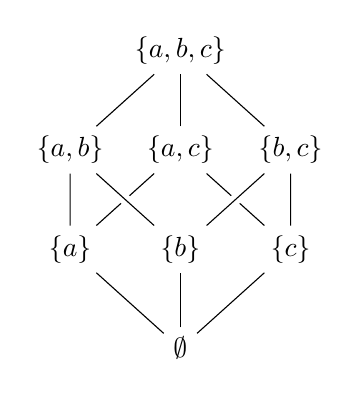
\begin{tikzpicture}[scale=0.7, yscale=0.9]
        \node (empty) at (0,0) {$\emptyset$};
        \node (a) at (-2,2) {$\{a\}$};
        \node (b) at (0,2) {$\{b\}$};
        \node (c) at (2,2) {$\{c\}$};
        \node (ab) at (-2,4) {$\{a,b\}$};
        \node (ac) at (0,4) {$\{a,c\}$};
        \node (bc) at (2,4) {$\{b,c\}$};
        \node (abc) at (0,6) {$\{a,b,c\}$};
        % Lines with no intersections
        \draw (empty) -- (a) -- (ab) -- (abc);
        \draw (empty) -- (c) -- (bc) -- (abc);
        \draw (empty) -- (b);
        \draw (ac) -- (abc);
        % Lines below
        \draw (a) -- (ac);
        \draw (c) -- (ac);
        % Lines above
        \draw[line width=4pt,draw=white] (b) -- (ab);
        \draw (b) -- (ab);
        \draw[line width=4pt,draw=white] (b) -- (bc);
        \draw (b) -- (bc);
    \end{tikzpicture}
    \caption{Hasse diagram for the power set $\powerset{\{a,b,c\}}$. Power sets are the most important class of (complete) lattices. In fact, they are \keyword{Boolean algebras}\index[subject]{Boolean algebra} since every element has a complement.}
\end{marginfigure}

If a set $A \subseteq P$ has a \emph{least} upper bound\index[subject]{upper bound!least|see{join}} $x$, then $x$ is called a \keyword{supremum}\index[subject]{supremum}\index[subject]{supremum|seealso{join}} or \keyword{join}\index[subject]{join} of $A$. A join of $A$ is determined up to equivalence if it exists, and we denote any such join by $\bigjoin A$\index[notation]{**-bigjoin@$\bigjoin$}. We similarly define an \keyword{infimum}\index[subject]{infimum}\index[subject]{infimum|seealso{meet}} or \keyword{meet}\index[subject]{meet} of $A$, denoted $\bigmeet A$\index[notation]{**-bigmeet@$\bigmeet$}, to be a greatest lower bound\index[subject]{lower bound!greatest|see{meet}} of $A$, if it exists. A join of a one- or two-element subset $\{x,y\}$ of $P$ is denoted $x \join y$\index[notation]{****-join@$\join$}, and we similarly write $x \meet y$\index[notation]{****-meet@$\meet$} for one of its meet.

Clearly two elements $x$ and $y$ has a join (resp. meet) in $P$ just when they have a meet (resp. join) in the dual $\dualord{P}$.

\begin{definition}[Lattices]
    Let $L$ be a poset. If $x \join y$ and $x \meet y$ exist for all $x,y \in L$, then $L$ is called a \keyword{lattice}\index[subject]{lattice}.
    %
    % \begin{enumdefinition}
    %     \item If $x \join y$ exists for all $x,y \in L$, then $L$ is called a \keyword{semilattice}.

    %     \item If $L$ and $\dualord{L}$ are both semilattices, then $L$ is called a \keyword{lattice}.

    %     \item If $\bigjoin A$ and $\bigmeet A$ exist for all $A \subseteq L$, then $L$ is called a \keyword{complete lattice}.
    % \end{enumdefinition}
\end{definition}
%
% What we call a semilattice is sometimes called a \emph{join}-semilattice, and $L$ is then called a \emph{meet}-semilattice if $\dualord{L}$ is a join-semilattice. But since these two properties are dual, it suffices to consider one of them. In particular, $L$ is a lattice if and only if $\dualord{L}$ is a lattice. Furthermore, if $L$ has all joins then it also has all meets, and vice-versa, since e.g. the meet of a set $A \subseteq L$ is the join of the set of lower bounds of $A$.
%
There\blfootnote{In standard first-order logic and universal algebra we usually require the underlying set of a structure or algebra to be nonempty (relaxing this assumption gets us into \keyword{free logic} territory, cf. \cite[Chapter~13]{priest-nonclassical-logic}). However, in algebra it is sometimes useful, or at least more natural, to allow domains to be empty: Otherwise the corresponding algebraic categories often have no initial object, and parallel morphisms with disjoint images have no equaliser.} is also an algebraic theory of lattices in which the operations $\join$ and $\meet$ are primary, and in which the order is defined using these operations (cf. \cite[Chapter~2]{davey-priestley-order}). Both approaches are equivalent.

Note also that authors differ on whether lattices must be nonempty, and even whether they must be bounded (in which case they cannot be empty): \Textcite[Definition~8.1]{schroeder-ordered-sets} allows empty lattices, \textcite[Definition~2.4]{davey-priestley-order} do not, and \textcite[§1.4]{johnstone-stone-spaces} requires lattices to be bounded.
% On the other hand, a complete lattice cannot be empty since the empty set is a subset of the lattice, and this must have both a join and a meet. Indeed, complete lattices are automatically bounded.


\subsection{Completeness in posets}

A\blfootnote{Let $\catC$ be a preorder category, i.e., a category with at most one arrow between a pair of objects. Then any pair of parallel arrows in $\catC$ have an equaliser, so for $\catC$ to be complete it suffices for it to have all products (cf. \cite[Proposition~5.1.26(a)]{leinster-category-theory} or any book on category theory). But products are precisely meets, so our terminology for posets is in agreement with the terminology from category theory.} preordered set $P$ is \keyword{complete}\index[subject]{preordered set!complete} if every subset of $P$ has a meet. If on the other hand $P$ has all joins, then we might have called $P$ \enquote{cocomplete}\index[subject]{preordered set!cocomplete}, if not for the fact that these properties are equivalent, as a standard argument shows.

Instead we are interested in preordered sets that do not have all joins, but that have \enquote{enough} joins, and specifically joins of particular kinds of subsets:

\begin{definition}
    Let $P$ be a poset, let $C \subseteq P$, and let $\kappa$ be a cardinal number. We say that
    %
    \begin{enumdefinition}
        \item $C$ is a \keyword{chain}\index[subject]{chain} if it is totally ordered.
        \item $C$ is a \keyword{$\kappa$-chain}\index[subject]{kappachain@$\kappa$-chain} if it is a chain and $\card{C} \leq \kappa$.
        \item $C$ is \keyword{consistent}\index[subject]{consistent set} if every finite subset of $C$ has an upper bound in $P$.
        \item $C$ is \keyword{directed}\index[subject]{directed set} if every finite subset of $C$ has an upper bound in $C$.
    \end{enumdefinition}
    %
    If $C$ has a join in $P$, then $C$ is called \keyword{convergent}\index[subject]{convergent set}.
\end{definition}
%
\blfootnote{By induction directedness of $D$ is equivalent to the property that, for every \emph{pair} of elements $x,y \in D$, there exists a $z \in D$ with $x \leq z$ and $y \leq z$, as long as $D$ is nonempty. This is the usual definition of directedness, but we prefer the \enquote{unbiased} version (cf. \cite{nlab:biased_definition}). Interestingly, some authors explicitly require both the existence of upper bound of finite subsets \emph{and} nonemptyness (cf. \cite[Definition~O-1.1]{gierz-continuous-lattices}), which of course is redundant.}%
%
A directed set is thus clearly consistent. Furthermore, if $P$ is topped then every subset is consistent, so this notion is only interesting if $P$ is not topped. If a set $\{x_1, \ldots, x_n\}$ is consistent then we also say that the $x_i$ are consistent.

Notice that a directed set $D$ is automatically nonempty, since the empty set is a finite subset of $D$. If $D$ is a directed set whose join exists, we often write $\bigdirjoin D \defeq \bigjoin D$\index[notation]{**-dirjoin@$\bigdirjoin$} instead. Another common notation is $\bigjoin^\uparrow D$\index[notation]{**-dirjoin2@$\bigjoin^\uparrow$}. We further note that the image of a chain, $\kappa$-chain, consistent or directed set under a monotone map also has this property.

For each type of subset of a poset, we may study special kinds of posets in which every such subset has a join. In the case of directed sets we in particular get the following:\blfootnote{In this setting what we call \enquote{cocompleteness} is often simply called \enquote{completeness}, but we follow \textcite{crole-categories-for-types} and prefer the category theory-friendly nomenclature.}

\begin{definition}
    Let $F$ be a property of subsets of posets. A poset $P$ is \keyword{$F$-cocomplete}\index[subject]{F-cocomplete@$F$-cocomplete} if every subset of $P$ with the property $F$ is convergent.
\end{definition}
%
For the most important choices of $F$ we use slightly altered terminology:
%
\begin{itemize}
    % \item When $F$ is \enquote{finite}, this just means that $P$ is a pointed semilattice.
    
    \item If $F$ is \enquote{bounded above}, then $P$ is \keyword{bounded cocomplete}\index[subject]{cocomplete!bounded}. If $P$ is nonempty then the empty set has an upper bound, and $P$ is automatically pointed. Some authors (e.g. \cite[Definition~5.7.3]{goubault-larrecq-topology}) build pointedness into their definition of bounded cocompleteness, while others (e.g. \cite[Definition~O-2.1(v)]{gierz-continuous-lattices}) do not but instead build nonemptyness into their definition of posets (cf. \cite[Definition~O-1.6]{gierz-continuous-lattices}). In \cref{def:Scott-domain} we define the class of posets of interest to us, and these posets will in either case be nonempty.

    \item Similarly, if $F$ is \enquote{consistent} then $P$ is \keyword{consistent cocomplete}\index[subject]{cocomplete!consistent}. Some authors also use the term \keyword{coherent} for $P$ in this case (e.g. \cite[Definition~1.2.28]{barendregt-lambda}).

    \item Most importantly, if $F$ is \enquote{directed}, then $P$ is \keyword{directed cocomplete}\index[subject]{cocomplete!directed} and is called a \keyword{\dCPO}\index[subject]{dcpo@\dCPO}. We obtain analogous properties if instead $F$ is \enquote{$\omega$-chain} or \enquote{chain}, in which case we respectively call $P$ an \keyword{\oCPO}\index[subject]{ocpo@\oCPO} or a \keyword{\cCPO}\index[subject]{ccpo@\cCPO}. We will focus on \dCPOpl{} in the sequel, but many results have analogous statements for the other types of complete posets. If any of the above are pointed, then we add an extra \enquote{p} to their abbreviations, so that we get \keyword{\oCPPO}\index[subject]{ocppo@\oCPPO}, \keyword{\cCPPO}\index[subject]{ccppo@\cCPPO} and \keyword{\dCPPO}\index[subject]{dcppo@\dCPPO}.
\end{itemize}

\begin{lemma}
    \label{lem:poset-completeness-equivalence}
    Let $P$ be a poset, and consider the following properties:
    %
    \begin{enumlemma}
        \item\label{enum:consistent-cocomplete} $P$ is consistent cocomplete.
        \item\label{enum:bounded-cocomplete} $P$ is bounded cocomplete.
        \item\label{enum:nonempty-meets-exist} $\bigmeet A$ exists for all nonempty $A \subseteq P$.
    \end{enumlemma}
    %
    Then the following implications hold:
    %
    \begin{equation*}
        \text{\itemref{enum:consistent-cocomplete}}
            \implies \text{\itemref{enum:bounded-cocomplete}}
            \iff \text{\itemref{enum:nonempty-meets-exist}}.
    \end{equation*}
    %
    If $P$ is a \dCPO{} then the implication \itemref{enum:bounded-cocomplete} $\implies$ \itemref{enum:consistent-cocomplete} also holds.
\end{lemma}

\begin{proof}
    The equivalence of \itemref{enum:bounded-cocomplete} and \itemref{enum:nonempty-meets-exist} is standard. Assuming \itemref{enum:consistent-cocomplete}, if $A \subseteq P$ is bounded above then it is automatically consistent. Finally, if $P$ is a \dCPO{} and \itemref{enum:bounded-cocomplete} holds, let $A \subseteq P$ be consistent and let $D \defeq \set{\bigjoin F}{F \subseteq_\omega A}$. Then $D$ is directed and it is easy to show that $\bigjoin A = \bigdirjoin D$.
\end{proof}



% \newcommand{\graph}[2][]{\calG\auxdelimparen[#1]{#2}}


% \begin{examplebreak}[Products of dcpo's]
%     Let $(P_i)_{i \in I}$ be a collection dcpo's, and equip the product $P \defeq \bigprod_{i \in I} P_i$ with the product order\footnote{The \keyword{product order} on $P = \bigprod_{i \in I} P_i$ is defined as follows: For $(x_i)_{i \in I}, (y_i)_{i \in I} \in P$ we say that $(x_i)_{i \in I} \leq (y_i)_{i \in I}$ if $x_i \leq y_i$ for all $i \in I$. The projections $\pi_i \colon P \to P_i$ are thus monotone, and, as an aside, we mention that $P$ is a categorical product in the category of posets and monotone maps.}. We claim that $P$ is also a dcpo. If $D \subseteq P$ is directed, then each $\pi_i\image{D}$ is also directed and thus has a join $x_i$. Letting $x = (x_i)_{i \in I}$ it is easy to see that $x = \bigdirjoin D$ in $P$: It is clear that $x$ is an upper bound of $D$, and furthermore $x \leq y$ if and only if $x_i \leq \pi_i(y)$ for all $y \in P$ and $i \in I$.

%     In particular,
%     %
%     \begin{equation*}
%         \pi_i \bigl( \bigdirjoin D \bigr)
%             = \pi_i(x)
%             = x_i
%             = \bigdirjoin \pi_i\image{D},
%     \end{equation*}
%     %
%     so $\pi_i$ is continuous.\footnote{It follows that $P$ is a product in the category of dcpo's and continuous maps.}
% \end{examplebreak}


\subsection{Algebraic posets and Scott domains}

\newcommand{\finite}[1]{F(#1)}
\newcommand{\waybelow}{\ll}

% \blfootnote{Finiteness is also sometimes, especially in algebra, called \keyword{compactness}. In a complete lattice $L$, an element $x \in L$ is also called compact if for every $A \subseteq L$ with $x \leq \bigjoin A$ there is a finite subset $A_0 \subseteq A$ such that $x \leq \bigjoin A$. This is equivalent to finiteness (cf. \cite[Lemma~7.16]{davey-priestley-order}) but of course requires completeness to make sense.}

\blfootnote{Finiteness also arises from the \enquote{way-below} relation: Given $x,y \in P$, if $y \leq \bigdirjoin D$ implies that $x \leq d$ for some $d \in D$, then $x$ is \keyword{way below}\index[subject]{way below} $y$, written $x \waybelow y$\index[notation]{***-waybelow@$\waybelow$}. Then $x$ is finite if and only if $x \waybelow x$. This notion leads to the theory of \keyword{continuous posets}\index[subject]{poset!continuous}, cf. \textcite[§5.1]{goubault-larrecq-topology}, a generalisation of algebraic posets.}

\begin{definition}[Finiteness]
    \label{def:poset-finite}
    Let $P$ be a poset. An element $x \in P$ is \keyword{finite}\index[subject]{finiteness (in posets)} if for all convergent directed $D \subseteq P$, if $x \leq \bigdirjoin D$ then there is a $d \in D$ with $x \leq d$. The set of finite elements of $P$ is denoted $\finite{P}$\index[notation]{fz-FP@$\finite{P}$}.
\end{definition}
%
Note that if $x$ and $y$ are finite, then $x \join y$ is also finite if it exists.
% It follows that if $P$ is a semilattice, then $\finite{P}$ is itself directed if it is nonempty (which is for instance the case if $P$ is pointed, since then the minimum of $P$ is finite).
Furthermore, if $x,y \in P$ with $x$ finite, then we write $x \leq_\omega y$\index[notation]{***-leqomega@$\leq_\omega$}. Since the finite elements of a power set are precisely those that are finite as sets, this notation is consistent with our notation \enquote{$\subseteq_\omega$} for finite subsets. % TODO finite notation, make commands

\begin{definition}[Algebraic posets]
    \label{def:algebraic-poset}
    A poset $P$ is \keyword{algebraic}\index[subject]{poset!algebraic} if
    %
    \begin{equation*}
        x
            = \bigdirjoin \set{y \in \finite{P}}{y \leq x}
    \end{equation*}
    %
    for all $x \in P$.
\end{definition}
%
Implicit in this definition is that the sets $\set{y \in \finite{P}}{y \leq x}$ are directed.
% Since $\finite{P}$ is closed under joins, this assumption is automatically satisfied if $P$ is a semilattice.


\begin{definition}[Scott domains]
    \label{def:Scott-domain}
    If $P$ is a \dCPPO{} that is algebraic and bounded cocomplete, then $P$ is called a \keyword{Scott domain}\index[subject]{Scott domain}.
\end{definition}
%
By \cref{lem:poset-completeness-equivalence} a Scott domain is automatically consistent complete.

\begin{marginfigure}\small
    \begin{tikzpicture}[scale=0.3]
        \tikzset{and so on edge/.style={dotted}} % TODO which style?
        \node (1) at (0,0) {$1$};
        \node (2) at (-2,-2) {$2$};
        \node (3) at (2,-2) {$3$};
        \node (more1) at (6,-2) {$\cdots$};
        \node (4) at (-4,-4) {$4$};
        \node (6) at (0,-4) {$6$};
        \node (9) at (4,-4) {$9$};
        \node (more2) at (8,-4) {$\cdots$};
        \node (0) at (0,-8) {$0$};
        \draw (1) -- (2) -- (4);
        \draw (1) -- (3) -- (9);
        \draw (1) -- (more1);
        \draw (2) -- (6);
        \draw (3) -- (6);
        \draw (4)[dash pattern=on 5pt off 5pt on 1pt off 2pt on 1pt off 2pt on 1pt off 2pt on 1pt off 2pt on 1pt off 5pt on 6pt] -- (0);
        \draw (6)[dash pattern=on 4pt off 4pt on 1pt off 2pt on 1pt off 2pt on 1pt off 4pt on 6pt] -- (0);
        \draw (9)[dash pattern=on 5pt off 5pt on 1pt off 2pt on 1pt off 2pt on 1pt off 2pt on 1pt off 2pt on 1pt off 5pt on 6pt] -- (0);
        \draw (0)[dash pattern=on 6pt off 5pt on 1pt off 2pt on 1pt off 2pt on 1pt off 2pt on 1pt off 2pt on 1pt off 2pt on 1pt off 2pt on 1pt off 2pt on 1pt off 2pt on 1pt off 2pt on 1pt off 2pt on 1pt off 2pt on 1pt off 2pt on 1pt off 2pt on 1pt off 2pt on 1pt off 2pt on 1pt off 2pt on 1pt] -- (more2);
    \end{tikzpicture}
    \caption{Hasse diagram for the lattice of subgroups of $\ints$, where a node $d$ represents the subgroup $d\ints$. Note that $1\ints = \ints$ and $0\ints = \{0\}$.}
    \label{fig:Z-subgroups}
\end{marginfigure}

\newcommand{\subalg}[1]{\operatorname{Sub}#1}

\begin{examplesbreak}
    \begin{enumexample}
        \item The lattice of subalgebras of an algebra (in the sense of universal algebra) is a complete algebraic lattice. For a concrete example, consider the group $(\ints,+)$: Its subgroups are $d\ints$ for $d \in \naturals$ (cf. \cite[Proposition~6.9]{aluffi-algebra-0}), and its lattice of subgroups is isomorphic to the dual $\dualord{(\naturals,\mid)}$\index[notation]{***-div@$\mid$ (divisibility)} of the naturals ordered by divisibility. This is depicted in \cref{fig:Z-subgroups}. % TODO number sets in introduction

        \item Any power set is also a complete algebraic lattice.

        \item\label{enum:pmaps-domain} If $X$ and $Y$ are sets, then the set $\pmaps{X}{Y}$ is a Scott domain: The finite elements in $\pmaps{X}{Y}$ are those partial maps with finite domain\footnote{If $f \in \pmaps{X}{Y}$ is a finite element, let $D$ be the set of the finite partial maps $d$ with $d \leq f$. Then $D$ is directed and $f = \bigdirjoin D$. The converse follows by induction on $\card{\dom{f}}$.}, and it is thus clear that $\pmaps{X}{Y}$ is algebraic. It is pointed with minimum $\bot$, and it is easy to see that it is a \dCPO. Finally, if $F \subseteq \pmaps{X}{Y}$ is bounded above, then taking the union of the graphs of the functions in $F$ yields the graph of partial map.
    \end{enumexample}
\end{examplesbreak}


\subsection{Topology}

\newcommand{\specorder}[1]{\Omega#1}

There are several different ways to equip an ordered set $P$ with a topology that somehow respect the ordering. Before surveying the options, consider the opposite problem, that of equipping a topological space with an ordering.

% \blfootnote{Given preordered sets $(P_i)_{i \in I}$, the \keyword{product order} on $\bigprod_{i \in I} P_i$ is given by $(x_i)_{i \in I} \leq (y_i)_{i \in I}$ if and only if $x_i \leq y_i$ for all $i \in I$. Equipped with this order, $\bigprod_{i \in I} P_i$ is a categorical product of the $P_i$ in the category of preordered sets. \par Similarly, the \keyword{coproduct order} on $\bigcoprod_{i \in I} P_i$ is given by $x \leq y$ if and only if $x,y \in P_i$ and $x \leq y$ in $P_i$ for some $i \in I$.}%
If $X$ is a topological space, define the \keyword{specialisation preorder}\index[subject]{specialisation preorder} $\preceq$ on $X$ by the condition that $x \preceq y$ if and only if every neighbourhood of $x$ is also a neighbourhood of $y$, or equivalently if $x \in \closure{\{y\}}$. The preordered set $(X,\preceq)$ is sometimes denoted $\specorder{X}$\index[notation]{ozzzz-OmegaX@$\specorder{X}$}.

This is a very natural ordering: For instance, $X$ is $T_0$ if and only if $\preceq$ is a partial order, and $X$ is $T_1$ is if and only if $\preceq$ is equality. More pertinent for us, every open set is upward closed in the specialisation preorder, and similarly every closed set is downward closed.
% Furthermore, the specialisation preorder on a product space is precisely the product of the specialisation preorders on each factor, and the same holds for coproducts (which are disjoint unions).

An obvious question is how the original order $\leq$ and the specialisation preorder $\preceq$ relate to each other. We have a useful criterion which the reader can readily check:

\begin{lemmanoproof}
    Let $(P,\leq)$ be a preordered set equipped with a topology, and let $\preceq$ be the specialisation preorder.
    %
    \begin{enumlemma}
        \item If every open set is upward closed with respect to $\leq$, then ${\leq} \subseteq {\preceq}$.
        \item If every principal lower set with respect to $\leq$ is closed, then ${\preceq} \subseteq {\leq}$.
    \end{enumlemma}
\end{lemmanoproof}


\subsubsection{Alexandroff topology}

\newcommand{\Alpha}{\mathrm{A}}
\newcommand{\Nu}{\mathrm{N}}

\newcommand{\alextop}[1]{\alpha(#1)}
\newcommand{\alexspace}[1]{\Alpha#1}
\newcommand{\uppertop}[1]{\nu(#1)}

\makeatletter
\def\upperspace{\@ifstar\@upperspace\@@upperspace}
\def\@upperspace#1{\Nu(#1)}
\def\@@upperspace#1{\Nu#1}
\makeatother

\newcommand{\scotttop}[1]{\sigma(#1)}
\newcommand{\scottspace}[1]{\Sigma#1}

\blfootnote{Given the set $S = \{0,1\}$ of truth values ordered by $0 < 1$, the space $\alexspace{S}$ is called the \keyword{Sierpi\'nski space}\index[subject]{Sierpinski space@Sierpi\'nski space}. It is well known that the functor $\calO \colon \dualcat{\catTop} \to \catSet$ sending a space to its topology is represented by $S$, so the restriction of $\calO$ to the category of ordered sets is also represented by $S$.}%
Given the above, an obvious way in which to equip a preordered set $(P,\leq)$ with a topology is just to let the open sets be the upward closed subsets of $P$. This is called the \keyword{Alexandroff topology}\index[subject]{Alexandroff topology} (also called the \keyword{specialisation topology}\index[subject]{specialisation topology}\index[subject]{specialisation topology|seealso{Alexandroff topology}}) on $P$, and is denoted $\alextop{P}$\index[notation]{azzzz-alphaP@$\alextop{P}$}, and the topological space $(P,\alextop{P})$ is denoted $\alexspace{P}$\index[notation]{azzzz-AlphaP@$\alexspace{P}$} (note that the \enquote{$\Alpha$} is a capital \enquote{$\alpha$}).

The specialisation preorder on $\alexspace{P}$ is precisely the original ordering on $P$ (i.e., $\specorder{\alexspace{P}} = P$)\footnote{In fact, one can show that there is an adjunction
%
\begin{equation*}
    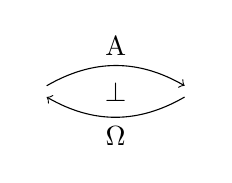
\begin{tikzpicture}[scale=0.5]
        \node (pre) at (0,0) {$\catPre$};
        \node (top) at (4,0) {$\catTop$};
        \node (adj) at (2,0) {$\bot$};
        \draw[->,bend left] (pre) to node[above] {$\alexspace{}$} (top);
        \draw[->,bend left] (top) to node[below] {$\specorder{}$} (pre);
    \end{tikzpicture}
\end{equation*}
%
where $\catPre$ is the category of preordered sets and monotone maps (cf. \cref{sec:ordered-sets-maps}). Note that $\specorder{}$ does not have a right adjoint since it does not preserve coequalisers: In both categories coequalisers are quotients, but while a quotient of a $T_1$-space is not necessarily $T_1$, a quotient of a discrete preordered set is still discrete.}, and it is easy to see that $\alextop{P}$ is the finest topology on $P$ with this property (cf. \cite[Proposition~4.2.11]{goubault-larrecq-topology}).

Furthermore, since the upward closed subsets of $P$ characterise its order by \cref{lem:order-vs-downsets}, we may recover the order from the topology.


\subsubsection{Upper topology}

There is also a \emph{coarsest} topology on $P$ that has the ordering on $P$ as its specialisation preorder. This is called the \keyword{upper topology}\index[subject]{upper topology} on $P$ and is denoted $\uppertop{P}$\index[notation]{nzzzz-nuP@$\uppertop{P}$}. The space $(P,\uppertop{P})$ is denoted $\upperspace{P}$\index[notation]{nzzzz-NuP@$\upperspace{P}$}. It is easy to check that $\uppertop{P}$ is indeed the coarsest such topology, once one has realised that $\closure{\{y\}} = \downset{y}$ with respect to the specialisation preorder. %\footnote{Some authors (e.g. \cite{andradi-ho-scott-convergence-theorem}) also denote this by $\Upsilon P$, which we find strangely inconsistent, while some authors (e.g. \cite{gierz-continuous-lattices}) do not reserve a symbol for it.}

More concretely, $\uppertop{P}$ has a subbasis consisting the sets $P \setminus \downset{x}$ for $x \in P$, or equivalently a basis consisting of the sets $P \setminus \downset{A}$ for finite subsets $A \subseteq P$ (cf. \cite[Proposition~4.2.12]{goubault-larrecq-topology}).


\subsubsection{Scott topology}

Neither the Alexandroff nor the upper topology is of much interest to us, but they help motivate the \keyword{Scott topology}\index[subject]{Scott topology}: We have already seen that directed subsets of posets have important properties, so we attempt to modify the Alexandroff topology to conform better to the directed subsets of $P$.

% TODO note Vickers!
Equip $P$ with a topology. Following \textcite{goubault-larrecq-topology}, let us think of open sets of $P$ as \enquote{tests}, such that an open set $U$ corresponds to the test \enquote{given $x \in P$, does $x \in U$?}. We further think of the ordering on $P$ as an \emph{information ordering}, in the sense that if $x \leq y$, then $y$ contains more information than $x$. This then implies that $U$ is upward closed, since if it is possible to determine that $x$ passes the test $U$, then it is also possible to determine that $y$ does because it contains all the information in $x$.

We next (informally) say that $U$ is \enquote{computable} if there is a computable partial function $f \colon P \pto \{0,1\}$ with the property that $f(x) = 1$ if and only if $x \in U$. Thinking of $f$ as a program $\pi$, it proceeds by considering \enquote{finite} parts $x_0,x_1,x_2,\ldots$ of $x$ such that the sequence $(x_n)_{n \in \naturals}$ \enquote{approximates} $x$. Since $x_n$ is supposed to be a better approximation of $x$ than $x_m$ if $m \leq n$, we suppose that the sequence $(x_n)_{n \in \naturals}$ is increasing. We interpret the idea that it approximates $x$ as $x = \bigjoin_{n \in \naturals} x_n$.

Given a test $U$ and the corresponding program $\pi$, if $\pi$ gets $x$ as input and outputs $1$, then it must have concluded that $x \in U$ on the basis of some approximation $x_n$. But then $x_n$ must itself pass the test $U$ since $x_n$ is precisely the part of $x$ that $\pi$ has used to conclude that $x \in U$. In other words, $x_n \in U$.%s Furthermore, the tail $x_{n+1},x_{n+2},\ldots$ must also lie in $U$ since these elements also contain the information in $x_n$.

This implies that $U$ should have the property that if $(x_n)_{n \in \naturals}$ is an increasing sequence whose join $x$ lies in $U$, then there is an $n \in \naturals$ such that $x_n$ already lies in $U$. Or put another way, if $C$ is a nonempty $\omega$-chain with $\bigjoin C \in U$, then $C \intersect U \neq \emptyset$.

However, it turns out that using $\omega$-chains leads to a theory that has some bizarre properties (cf. \cite[§2.2.4]{abramsky-jung-domain-theory}). Hence it is customary to instead use \emph{directed sets}, even though these do not exactly model the way in which a program executes. Thus we arrive at the following definition:

\begin{definition}
    Let $P$ be a poset. A subset $U \subseteq P$ is said to be \keyword{inaccessible}\index[subject]{inaccessible set} if $\bigdirjoin D \in U$ implies $D \intersect U \neq \emptyset$ for all convergent directed sets $D \subseteq P$.
\end{definition}
%
The \keyword{Scott topology}\index[subject]{Scott topology} on $P$ then consists of all the inaccesible upper sets. We denote it $\scotttop{P}$\index[notation]{szzzz-sigmaP@$\scotttop{P}$}, and the space $(P,\scotttop{P})$ is denoted $\scottspace{P}$\index[notation]{szzzz-SigmaP@$\scottspace{P}$}. This also has the property that the specialisation preorder on $\scottspace{P}$ is precisely the original ordering on $P$, implying that $\scotttop{P}$ lies (usually strictly) between $\alextop{P}$ and $\uppertop{P}$: simply notice that every principal lower set is Scott closed (cf. \cite[Proposition~4.2.18]{goubault-larrecq-topology}).



% Let $\calO$ be the collection of subsets of $P$ that are upward closed and inaccessible by directed joins. Then $\calO$ is closed under arbitrary unions, since if $D \subseteq P$ is convergent and directed and $\bigdirjoin D \in \bigunion_{i \in I} U_i$ with $U_i \in \calO$, then $\bigdirjoin D \in U_i$ for some $i$, and hence $\emptyset \neq D \intersect U_i \subseteq D \intersect \bigunion_{i \in I} U_i$. Similarly, if $U,V \in \calO$ and $\bigdirjoin D \in U \intersect V$, then there are elements $x \in D \intersect U$ and $y \in D \intersect V$. And since $D$ is directed $x$ and $y$ have an upper bound $z$ in $D$, and since $U$ and $V$ are upward closed we have $z \in U \intersect V$. That is, $\calO$ is a topology on $P$:

% \begin{definition}[Scott topology]
%     Let $P$ be a poset. The family of subsets that are upward closed and inaccessible by directed joins is called the \keyword{Scott topology} on $P$.
% \end{definition}

% % It is useful to note that a subset $F \subseteq P$ is closed in e.g. the directed Scott topology if and only if is downward closed and $\bigdirjoin D \in F$ for all directed subsets $D \subseteq F$. Note that if $x \in P$, then $\downset{x}$ is closed: It is clearly downward closed, and $x$ is an upper bound of every subset $A \subseteq \downset{x}$, so the join of $A$ (if it exists) also lies in $\downset{x}$. % TODO is this necessary?






% We similarly find that the collections of subsets of $P$ that are upwards closed and inaccessible by joins of ($\kappa$-)chains also constitute topologies on $P$. % TODO


\subsubsection{Pointwise convergence}

\blfootnote{In the complete lattice $[0,1]$ with the usual order, only $0$ is finite. On the other hand, it is easy to see that $\upset{x}$ is accessible for all $x \in (0,1]$. \par Or a less trivial example: In the complete lattice $C$ of closed subsets of $\reals$, where meet is intersection and join is union followed by closure, infinite closed sets are not finite in $C$. For instance,
%
\begin{equation*}
    \bigdirjoin_{n \in \posints} [\tfrac{1}{n},1]
        = [0,1],
\end{equation*}
%
so $[0,1]$ is not finite. Hence $\upset{[0,1]}$ is accessible.}

% \begin{lemma}
%     \label{lem:finite-inaccessible}
%     If $P$ is a poset and $x \in P$, then $\upset{x}$ is inaccessible if and only if $x$ is finite in $P$.
% \end{lemma}

% \begin{proof}
%     This follows directly from the definitions since $x \leq \bigdirjoin D$ if and only if $\bigdirjoin D \in \upset{x}$.
% \end{proof}

If $x \in P$ is finite, then we easily check that $\upset{x}$ is inaccessible and hence Scott open. Hence the principal upper sets in $P$ constitute subcollection of the Scott topology. Letting these induce a topology we get the following:

\begin{definition}[Topology of pointwise convergence]\index[subject]{topology of pointwise convergence}
    Let $P$ be a poset. The topology on $P$ generated by
    %
    \begin{equation*}
        \set{x^\uparrow}{x \in \finite{P}}
    \end{equation*}
    %
    is called the \keyword{topology of pointwise convergence}.
\end{definition}
%
That is, $\set{x^\uparrow}{x \in \finite{P}}$ is a subbasis for the topology. It gets its name from its main application in domains of partial maps, as we return to in \cref{sec:partial-maps}.
% If $P$ is a semilattice, then this subbasis is closed under intersection and is thus in fact a basis for the topology: For note that if $x,y \in P$ has a join, then this join is also finite, and we clearly have $\upset{x} \intersect \upset{y} = \upset*{x \join y}$.

The topology of pointwise convergence is generally strictly coarser than the Scott topology\footnote{In $[0,1]$ the only finite element is $0$, so the topology of pointwise convergence is trivial. On the other hand, any subset $(x,1]$ is inaccessible. In general, sets on the form $\upset{x} \setminus \{x\}$ provide counterexamples in many \dCPOpl.}, but in many important posets the two coincide:

\begin{proposition}
    \label{prop:Scott-topology-pointwise-equal}
    If $P$ is an algebraic poset, then the Scott topology and the topology of pointwise convergence on $P$ coincide.
\end{proposition}

\begin{proof}
    Let $U$ be a Scott open subset of $P$, and let $x \in U$. Since $P$ is algebraic we have $x = \bigdirjoin \set{y \in \finite{P}}{y \leq x}$, and since $U$ is inaccessible there is a $y \leq_\omega x$ in $U$. Finally, since $U$ is upward closed we have $\upset{y} \subseteq U$, so in total
    %
    \begin{equation*}
        U
            = \bigunion_{y \in U \intersect \finite{P}} \upset{y}.
    \end{equation*}
    %
    Thus $U$ is also open in the topology of pointwise convergence.
\end{proof}


\section{Arrows}

\subsection{Maps between ordered sets}\label{sec:ordered-sets-maps}

\begin{definition}
    Let $P$ and $Q$ be preordered sets. A map $f \colon P \to Q$ is said to be \keyword{monotone}\index[subject]{monotone map} if $x \leq y$ implies $f(x) \leq f(y)$ for all $x,y \in P$.
\end{definition}
%
Clearly the composition of two monotone maps is monotone, and the identity map is monotone, so this yields a category $\catPre$ of preordered sets and monotone maps.

We have the following characterisation of monotonicity which the reader can readily check:

\begin{propositionnoproof}
    \label{prop:monotone-upward-downward-closed}
    Let $P$ and $Q$ be preordered sets and let $f \colon P \to Q$ be a function. Then the following are equivalent:
    %
    \begin{enumproposition}
        \item $f$ is monotone.
        \item If $B \subseteq Q$ is upward closed, then $f\preim{B}$ is also upward closed.
        \item If $B \subseteq Q$ is downward closed, then $f\preim{B}$ is also downward closed.
    \end{enumproposition}
\end{propositionnoproof}

% \begin{proof}
%     First assume that $f$ is monotone, let $B \subseteq Q$ be upward closed, and let $y \in f\preim{B}$. If $x \leq y$, then $f(x) \leq f(y)$, and so $f(x) \in B$. But then $x \in f\preim{B}$ as required.

%     Conversely assume that the preimage under $f$ of an upward closed set is upward closed, and let $x,y \in P$ with $x \leq y$. Then $\downset{f(y)}$ is downward closed, and hence so is $f\preim{\downset{f(y)}}$. But then $x \in f\preim{\downset{f(y)}}$, so $f(x) \in \downset{f(y)}$, implying that $f(x) \leq f(y)$.

%     Since the complement of an upward closed set is downward closed, and vice-versa, the last two properties are clearly equivalent.
% \end{proof}


% \begin{definition}[Lattice homomorphisms]
%     Let $L$ and $K$ be semilattices, and let $f \colon L \to K$ be if $f(x \join y) = f(x) \join f(y)$ for all $x,y \in L$, then $f$ is a \keyword{semilattice homomorphism}. If $L$ and $K$ are lattices and also $f(x \meet y) = f(x) \meet f(y)$ for all $x,y \in L$, then $f$ is called a \keyword{lattice homomorphism}. In each case $f$ is an \keyword{isomorphism} if it is invertible and both $f$ and $f\inv$ are homomorphisms.
% \end{definition}


% There is of course a relationship between monotone maps and lattice homomorphisms: We have the following result, whose proof is trivial, that all semilattice homomorphisms are monotone, and that monotone maps are \enquote{halfway} to being lattice homomorphisms.

% \begin{lemmanoproof} % TODO do I need this?
%     If $L$ and $K$ are lattices and $f \colon L \to K$ is a map, then the following are equivalent:
%     %
%     \begin{enumlemma}
%         \item $f$ is monotone,
%         \item $f(x \join y) \geq f(x) \join f(y)$ for all $x,y \in L$, and
%         \item $f(x \meet y) \leq f(x) \meet f(y)$ for all $x,y \in L$.
%     \end{enumlemma}
% \end{lemmanoproof}




% Note that if $f$ is instead order-reversing, then since the corresponding map $L \to \dualord{K}$ is monotone, we have e.g.
% %
% \begin{equation*}
%     f(x \join y) \dualord{\geq} f(x) \dualord{\join} f(y),
% \end{equation*}
% %
% implying that
% %
% \begin{equation*}
%     f(x \join y) \leq f(x) \meet f(y).
% \end{equation*}
% %
% The following application of this fact will be useful later. % TODO do I need this?

% \begin{example}
%     \label{ex:upset-of-join}
%     In this example, given a map $f \colon P \to Q$ between posets, we denote by $\dualord{f}$ the map $\dualord{P} \to Q$ given by $\dualord{f}(x) = f(x)$.

%     Let $(P,\leq)$ be a poset, and consider the map $d_P \colon P \to \powerset{P}$ given by $d_P(x) = \downset{x}$, which is clearly an order-embedding. If $P$ is a meet semilattice, then $d_P$ in fact preserves meets, i.e., is a meet semilattice homomorphism: For if $z \in (x \meet y)^\downarrow$, then $z$ is smaller than both $x$ and $y$, and hence an element in both $\downset{x}$ and $y^\downarrow$.

%     Consider also the map $u_P \colon P \to \powerset{P}$ given by $u_P(x) = \upset{x}$. It is then easy to show that $\dualord*{u_P} = d_{\dualord{P}}$, so this is monotone. If $P$ is a join semilattice with join $\join$, then $\dualord{P}$ is a meet semilattice, and the above implies that $\dualord*{u_P}$ is a meet semilattice homomorphism. This means that for $x,y \in P$, we have
%     %
%     \begin{equation*}
%         \dualord*{u_P}(x \dualord{\meet} y)
%             = \dualord*{u_P}(x) \intersect \dualord*{u_P}(y).
%     \end{equation*}
%     %
%     Since $\dualord*{u_P}(x) = u_P(x) = \upset{x}$, this just means that
%     %
%     \begin{equation*}
%         (x \join y)^\uparrow
%             = \upset{x} \intersect y^\uparrow,
%     \end{equation*}
%     %
%     which is also easy to verify directly.
% \end{example}







\subsection{Continuity}

If $P$ and $Q$ are preordered sets, then it follows directly from \cref{prop:monotone-upward-downward-closed} that a map $f \colon P \to Q$ is monotone if and only if it is continuous with respect to the Alexandroff topology. If $f$ instead is continuous with respect to the Scott topology, then $f$ is called \keyword{Scott continuous}\index[subject]{Scott continuous map}.

\begin{lemma}
    \label{lem:Scott-continuous-monotone}
    If $f \colon P \to Q$ is Scott continuous, then $f$ is monotone and hence continuous with respect to the Alexandroff topology.
\end{lemma}

\begin{proof}
    Let $x,y \in P$ with $x \leq y$. The set $\downset{f(y)}$ is closed in $Q$, so its preimage $f\preim{\downset{f(y)}}$ is closed in $P$ and is in particular downward closed. Hence it contains $x$, and so $f(x) \in \downset{f(y)}$, which means that $f(x) \leq f(y)$.
\end{proof}



% \begin{examplebreak}[Partial functions]
%     If $X$ and $Y$ are sets, then we order the set $\pmaps{X}{Y}$ of partial functions as follows: For $f,g \colon X \pto Y$ we let $f \leq g$ if $\dom f \subseteq \dom g$ and $f(x) = g(x)$ for all $x \in \dom f$. The \keyword{graph} of a partial function $f$ is the set
%     %
%     \begin{equation*}
%         \graph{f} = \set{(x,y) \in X \prod Y}{x \in \dom f \text{ and } f(x) = y}.
%     \end{equation*}
%     %
%     This induces a map $\calG \colon \pmaps{X}{Y} \to \powerset{X \prod Y}$ given by $f \mapsto \graph{f}$, which is clearly an order-embedding. If $D \subseteq \pmaps{X}{Y}$ is a directed set of partial functions, then it is clear that the set $\bigdirjoin \calG\image{D} = \bigunion_{d \in D} \graph{d}$ is the graph of a partial function. This function is then the join of $D$ in $\pmaps{X}{Y}$, which is therefore a \dCPO, and the map $\calG$ is thus continuous. In fact, $\pmaps{X}{Y}$ is pointed since the empty map is the least element.

%     Denoting the projection maps by $\pi_X \colon X \prod Y \to X$ and $\pi_Y \colon X \prod Y \to Y$, notice that $\dom f = \pi_X\image{\graph{f}}$ and $\ran f = \pi_Y\image{\graph{f}}$. Since images preserve unions, and joins in power sets are just unions, if $D \subseteq \pmaps{X}{Y}$ is directed then
%     %
%     \begin{equation*}
%         \dom \bigdirjoin D
%             = \pi_X\image[\big]{\graph[\big]{\bigdirjoin D}}
%             = \pi_X\image[\big]{\bigdirjoin \calG\image{D}}
%             = \bigdirjoin \pi_X\image[\big]{\calG\image{D}}
%             = \bigdirjoin \dom\image{D},
%     \end{equation*}
%     %
%     and we similarly have $\ran \bigdirjoin D = \bigdirjoin \ran\image{D}$.
% \end{examplebreak}




There is a different characterisation of continuous maps between posets. If $f \colon P \to Q$ is a map between posets, then we say that $f$ \keyword{preserves joins}\index[subject]{preservation!of joins} if whenever $\bigjoin A$ exists in $P$ for a subset $A \subseteq P$, then $\bigjoin f\image{A}$ exists in $Q$ and $f(\bigjoin A) \equiv \bigjoin f\image{A}$. We often consider slightly different properties where we require $f$ to preserve certain properties of subsets as well as joins of subsets with these properties. For instance, we say that\blfootnote{A function that preserves directed joins is also often called continuous, but we reserve this name for functions that are continuous in the topological sense.} $f$ \keyword{preserves directed joins}\index[subject]{preservation!of directed joins} if, whenever $D \subseteq P$ is directed and $\bigdirjoin D$ exists in $P$, then $f\image{D}$ is also directed, $\bigdirjoin f\image{D}$ exists in $Q$ and $f(\bigdirjoin D) \equiv \bigdirjoin f\image{D}$. We then have the following:

% \begin{lemma}
%     \label{lem:continuous-monotone}
%     If $f \colon P \to Q$ is continuous, then $f$ is monotone.
% \end{lemma}

% \begin{proof}
    % If $x,y \in P$ with $x \leq y$, then $\{x,y\}$ is a directed set with $\bigdirjoin \{x,y\} = y$, and so $f(y) = \bigdirjoin \{f(x),f(y)\}$. In particular, $f(x) \leq f(y)$.
% \end{proof}

% However, while continuous functions are automatically Scott continuous, the converse does not generally hold. But making appropriate assumptions about the underlying posets we get the following:

\begin{proposition}
    \label{prop:continuous-vs-Scott-continuous}
    Let $P$ and $Q$ be preordered sets. A map $f \colon P \to Q$ preserves directed joins if and only if it is Scott continuous.
\end{proposition}

\begin{proof}
    First\blfootnote{This result gives another interpretation of the Scott topology: Namely the one in which a set $U$ is open just when the characteristic function $\chi_U \colon P \to S$ preserves directed joins. (Here $S = \{0,1\}$ is the set of truth values with $0 < 1$, as defined above.)}
    assume that $f$ preserves directed joins, and let $F \subseteq Q$ be closed in the Scott topology. Assume that $D \subseteq f\preim{F}$ is convergent and directed. Then $f\image{D} \subseteq F$, so
    %
    \begin{equation*}
        f \Bigl( \bigdirjoin D \Bigr)
            = \bigdirjoin f\image{D}
            \subseteq F,
    \end{equation*}
    %
    which implies that $\bigdirjoin D \in f\preim{F}$. We easily see that $f$ is monotone, so \cref{prop:monotone-upward-downward-closed} implies that $f\preim{F}$ is also downward closed, hence closed in the Scott topology.
    %\footnote{If $x,y \in P$ with $x \leq y$, then $\{x,y\}$ is a directed set with $\bigdirjoin \{x,y\} = y$, and so $f(y) = \bigdirjoin \{f(x),f(y)\}$. In particular, $f(x) \leq f(y)$.}

    Conversely assume that $f$ is Scott continuous, and let $D \subseteq P$ be convergent and directed. By \cref{lem:Scott-continuous-monotone} $f$ is monotone, so $f(\bigdirjoin D)$ is an upper bound of $f\image{D}$. If $x$ is any upper bound of $f\image{D}$, then $f\image{D} \subseteq \downset{x}$, implying that $D \subseteq f\preim{\downset{x}}$. But since $\downset{x}$ is Scott closed so is $f\preim{\downset{x}}$, and hence $\bigdirjoin D \in f\preim{\downset{x}}$. This just means that $f(\bigdirjoin D) \in \downset{x}$, so $f(\bigdirjoin D) \leq x$ as required.
\end{proof}


% If $X$ and $Y$ are topological spaces, then strengthening the topology on $X$ and weakening the topology on $Y$ yields a (potentially) larger collection of continuous maps $X \to Y$, and vice versa. But either strengthening or weakening both topologies simultaneously does not generally have a predictable effect on the set of continuous maps, even if we can somehow strengthen or weaken both topologies in a \enquote{uniform} way. In the present case, however, it turns out that Scott continuity implies continuity with respect to the other two Scott-like topologies: that is, the ones in which open sets are those that are upward closed and inaccessible by joins of $\omega$-chains or arbitrary chains. This follows immediately from \cref{prop:continuous-vs-Scott-continuous} since every $\omega$-chain is a chain, and every chain is directed. % TODO

% \begin{convention}
%     If $P$ and $Q$ are \dCPOpl, then a map $f \colon P \to Q$ is simply called \keyword{continuous} if it is Scott continuous, or equivalently it preserves directed joins.
% \end{convention} % TODO?


% \subsection{Algebraic maps}

% \begin{definition}
%     Let $P$ and $Q$ be posets. A monotone map $f \colon P \to Q$ is \keyword{algebraic} if
%     %
%     \begin{equation*}
%         f(x)
%             = \bigjoin \set{f(y)}{y \in \finite{P} \text{ and } y \leq x}
%     \end{equation*}
%     %
%     for all $x \in P$.
% \end{definition}
% %
% Note that if $\finite{P}$ is directed, then the set on the right-hand side is also since $f$ is monotone.


% \begin{proposition}
%     \label{prop:algebraic-vs-continuous}
%     Let $P$ and $Q$ be posets, and let $f \colon P \to Q$. If $f$ is algebraic, then it preserves directed joins. The converse also holds if $P$ is algebraic.
% \end{proposition}

% \begin{proof}
%     First assume that $f$ is algebraic, and let $D \subseteq P$ be a convergent directed subset. If $y \in P$ is finite and $y \leq \bigdirjoin D$, then there is some $d \in D$ with $y \leq d$, implying that $f(y) \leq f(d)$. We thus have
%     %
%     \begin{align*}
%         f \Bigl( \bigdirjoin D \Bigr)
%             &= \bigjoin \set[\Big]{f(y)}{y \in \finite{P} \text{ and } y \leq \bigdirjoin D} \\
%             &\leq \bigdirjoin \set{f(d)}{d \in D} \\
%             &= \bigdirjoin f\image{D}.
%     \end{align*}
%     %
%     The opposite inequality always holds, so the claim follows.

%     Conversely assume that $P$ is algebraic, and assume that $f$ preserves directed joins. Consider $x \in P$ and let $D \defeq \set{y \in \finite{P}}{y \leq x}$, so that $x = \bigdirjoin D$. Then we have
%     %
%     \begin{equation*}
%         f(x)
%             = f \Bigl( \bigdirjoin D \Bigr)
%             = \bigdirjoin f\image{D}
%             = \bigdirjoin \set{f(y)}{y \in \finite{P} \text{ and } y \leq x},
%     \end{equation*}
%     %
%     which precisely says that $f$ is algebraic.
% \end{proof}
% %
% We sum up the relationship between being algebraic, Scott continuous, and preserving directed joins in \cref{fig:continuity-overview}.

% \begin{figure}\small
%     \begin{sidecaption}{Relationship between properties of maps between posets. The leftmost implications follow from \cref{prop:algebraic-vs-continuous}, and the rightmost from \cref{prop:continuous-vs-Scott-continuous}.}[fig:continuity-overview]
%         \centering
%         \begin{tikzpicture}
%             % \tikzset{implies edge/.style={-implies,double equal sign distance}}
%             \tikzset{implies edge/.style={->}}
%             \node (alg) at (0,0) {algebraic};
%             \node (joins) at (4,0) [align=center] {preserves\\ dir. joins};
%             \node (Scott) at (8,0) [align=center] {Scott \\ continuous};
%             \draw[implies edge] (alg) to [bend left] (joins);
%             \draw[implies edge] (joins) to [bend left] (Scott);
%             \draw[implies edge] (Scott) to [bend left] node[below]{\dCPO} (joins);
%             \draw[implies edge] (joins) to [bend left] node[below]{algebraic poset} (alg);
%         \end{tikzpicture}
%     \end{sidecaption}
% \end{figure}




\subsection{Expansive maps}

This section is only needed in the proof of \cref{thm:Zermelo}. Readers can on a first pass skip this section and return to it as needed.

A map $f \colon P \to P$ on a poset $P$ is called \keyword{expansive}\index[subject]{expansive map} if $x \leq f(x)$ for all $x \in P$. The following lemma describes how we in some cases can restrict $f$ to a particularly nice subset of $P$ on which $P$ is monotone.
% \blfootnote{Some authors also use the adjectives \keyword{extensive}, \keyword{inflationary} or even \keyword{increasing}.}

\blfootnote{A \keyword{sub-\cCPO{}}\index[subject]{subccpo@sub-\cCPO} $Q$ of $P$ is a subset of $P$ such that if $C$ is a chain in $Q$ with join $\bigjoin C \in P$, then $\bigjoin C$ also lies in $Q$. Furthermore, $Q$ is a \keyword{sub-\cCPPO{}}\index[subject]{subccppo@sub-\cCPPO} of $P$ if the bottom element of $P$ also lies in $Q$.}

\begin{lemma}
    \label{lem:expansive-gives-monotone}
    Let $P$ be a \cCPPO{} and $f \colon P \to P$ be expansive. If $P_0$ is the smallest $f$-invariant sub-\cCPPO{} of $P$, then $P_0$ is a chain and $f|_{P_0}$ is monotone. In particular, $P_0$ is bounded.\footnote{This result is adapted from \textcite[Exercise~8.20]{davey-priestley-order}.}
\end{lemma}

\begin{proof}
    We will call an element $x \in P_0$ a \enquote{roof} if $y < x$ implies $f(y) \leq x$ for all $y \in P_0$. For a roof $x$ we consider the set
    %
    \begin{equation*}
        Z_x
            = \set{y \in P_0}{y \leq x \text{ or } f(x) \leq y}.
    \end{equation*}
    %
    We claim that $Z_x$ is an $f$-invariant \cCPPO, so let $y \in Z_x$. If $y \leq x$, then either $y = x$ in which case $f(x) \leq f(y)$, or else $y < x$ so that $f(y) \leq x$ since $x$ is a roof. If instead $f(x) \leq y$, then since $f$ is expansive we have $f(x) \leq f(y)$. Hence $f(y) \in Z_x$, so $Z_x$ is $f$-invariant. Next let $C \subseteq Z_x$ be a chain. If $y \leq x$ for all $y \in x$, then we also have $\bigjoin C \subseteq x$. If instead there is some $y \in C$ with $f(x) \leq y$, then we clearly have $f(x) \leq \bigjoin C$. Thus $Z_x$ is a \cCPPO, so by minimality of $P_0$ we have $P_0 = Z_x$.

    Next we claim that every element in $P_0$ is a roof. Consider the set
    %
    \begin{equation*}
        Z
            = \set{x \in P_0}{\text{$x$ is a roof}}.
    \end{equation*}
    %
    We show that $Z$ is an $f$-invariant \cCPPO. If $x$ is a roof and $y \in P_0$, then $y \in Z_x$ and so either $y \leq x$ or $f(x) \leq y$. If $y < f(x)$ then we must have $y \leq x \leq f(x)$, so that $f(x)$ is also a roof, and so $Z$ is $f$-invariant. If $C \subseteq Z$ is a chain and $y < \bigjoin C$, then there is some $x \in C$ with $y < x \leq \bigjoin C$, so $Z$ is also chain cocomplete. Again by minimality we have $P_0 = Z$.

    Now notice that $P_0$ is a chain: If $x,y \in P_0$, then $x$ is a roof and so $y \in Z_x$, which implies that either $y \leq x$ or $x \leq f(x) \leq y$. If $x < y$, then necessarily $f(x) \leq y \leq f(y)$, so $f$ is monotone on $P_0$. Finally, since itself $P_0$ is a chain the join $\bigjoin P_0$ lies in\footnote{This is where we use that $P$ is chain cocomplete and not just $\omega$-chain cocomplete, since $P_0$ may be uncountable. The rest of the proof goes through with this weaker assumption (with \enquote{\cCPPO} replaced with \enquote{\oCPPO}), but we shall not need this fact.} $P_0$ and is its maximum.
\end{proof}



\section{Posets of partial maps}\label{sec:partial-maps}

Recall from \cref{enum:pmaps-domain} that a set $\pmaps{X}{Y}$ of partial maps is a Scott domain whose finite elements are the finite partial maps. Unless $Y$ is a singleton (or $X$ is empty), $\pmaps{X}{Y}$ is not topped: If $x \in X$ and $y_1,y_2 \in Y$ are distinct, then any maps with $x \mapsto y_1$ and $x \mapsto y_2$ respectively are inconsistent.


% Recall that we order the set $\pmaps{X}{Y}$ of partial maps by the inclusion order on the graphs of its elements.

% \begin{lemma}
%     A partial map $f \colon X \pto Y$ is finite (cf. \cref{def:poset-finite}) in $\pmaps{X}{Y}$ if and only if its domain $\dom f$ is a finite set, i.e., if $\dom f$ is finite in $X$.\footnote{This is a generalisation of \textcite[Lemma~6.28]{moschovakis-set-theory}.}
% \end{lemma}

% \begin{proof}
%     First assume that $\dom f$ is finite, and let $D \subseteq \pmaps{X}{Y}$ be directed. The proof is by induction on the number of elements in $\dom f$. If this domain is empty, then the claim is obvious, so assume that $\dom f$ has $n+1$ elements. If $x \in \dom f$, then there is a map $f_1$ such that $f = f_1 \join f|_{\{x\}}$, and $\dom f_1$ has $n$ elements. By induction there is a $d' \in D$ with $f_1 \leq d'$, and there furthermore must be some $d'' \in D$ with $f|_{\{x\}} \leq d''$. By directedness there is some $d \in D$ greater than both $d'$ and $d''$, so $f \leq d' \join d'' \leq d$ as desired.

%     Conversely assume that $f$ is finite in $\pmaps{X}{Y}$, and let $D$ be the set of partial maps $d$ with finite domain such that $d \leq f$. Then $D$ is clearly directed and $f = \bigdirjoin D$, so there is some $d \in D$ such that $f \leq d$. But then the domain of $f$ must be finite, as claimed.
% \end{proof}

% If partial functions $f,h \colon X \pto Y$ satisfy $f \leq h$, then we say that $h$ is an \keyword{extension} of $f$. If also $g \leq h$ for some $g \colon X \pto Y$, then we clearly have $f \join g \leq h$, so $h$ is a \emph{common} extension of $f$ and $g$. This is of course the case just when $h \in (f \join g)^\uparrow$. Recall that $(f \join g)^\uparrow = f^\uparrow \intersect g^\uparrow$ from \cref{ex:upset-of-join}, which in this context simply means that $h$ is a common extension of $f$ and $g$ just when $h$ is both an extension of $f$ and of $g$.

% Since the join of two finite elements is finite, the collection $\set{f^\uparrow}{f \colon X \pto_\omega Y}$ is closed under binary intersections. It is thus a basis for a topology on $\pmaps{X}{Y}$:

% \begin{definition}[Topology of pointwise convergence]
%     Let $X$ and $Y$ be sets. The topology on $\pmaps{X}{Y}$ generated by the basis
%     %
%     \begin{equation*}
%         \set{f^\uparrow}{f \colon X \pto_\omega Y}
%     \end{equation*}
%     %
%     is called the \keyword{topology of pointwise convergence}.
% \end{definition}

\subsection{Topology}\label{sec:pmaps-topology}

Recall that\blfootnote{Note that the name \enquote{topology of pointwise convergence} is usually given to the product topology on the set $\tmaps{X}{Y}$ of total maps, when $Y$ is a topological space. In this case \enquote{pointwise} means that a sequence $(f_n)_{n \in \naturals}$ (or more generally a net) in $\tmaps{X}{Y}$ converges to a function $f$ if and only if the sequences $(f_n(x))_{n \in \naturals}$ converge to $f(x)$ for all $x \in X$.} on $\pmaps{X}{Y}$ the Scott topology and topology of pointwise convergence coincide by \cref{prop:Scott-topology-pointwise-equal}. In this context we can better explain the meaning of \enquote{pointwise convergence}: If $(f_i)_{i \in I}$ is a sequence in $\pmaps{X}{Y}$ which converges to some $f \colon X \pto Y$, then this means that for every $g \leq_\omega f$ there exists an $i_0 \in I$ such that $i \geq i_0$ implies $g \leq f_i$. Since such a map $g$ is uniquely determined by its domain, this just says that for every $A \subseteq_\omega \dom f$ there is such an $i$ with $f_i|_A = f|_A$ when $i \geq i_0$. That is, the functions in the sequence eventually agree with $f$ on arbitrarily large, but finite, subsets of $X$.

On the other hand, every partial map $f$ can be approximated by finite maps, though unless we know more about the structure of $X$ we cannot necessarily approximate $f$ with a \emph{sequence}. Let $\calA = \powersetfin{\dom{f}}$ and let $f_A = f|_A$. Then $(f_A)_{A \in \calA}$ is a net, and it is clear that it converges to $f$.

% \newcommand{\ev}[1][]{\mathrm{ev}_{#1}}
\newcommand{\ev}[1][]{\epsilon_{#1}}

Let $*$ be some element disjoint from $Y$, and let $Y_* \defeq Y \union \{*\}$. Every $f \colon X \pto Y$ gives rise to a total function $f_* \colon X \to Y_*$ by
%
\begin{equation*}
    f_*(x) =
    \begin{cases}
        f(x), & x \in \dom{f}, \\
        *,    & x \not\in \dom{f}.
    \end{cases}
\end{equation*}
%
This map clearly induces a bijection $\pmaps{X}{Y} \bijto \tmaps{X}{Y_*}$ given by $f \mapsto f_*$. Furthermore, for $x \in X$ define $\ev[x] \colon \pmaps{X}{Y} \to Y_*$ by $\ev[x](f) = f_*(x)$. We then have the following result:

\begin{proposition}
    Equip $Y_*$ with the discrete topology. Then $\pmaps{X}{Y}$ along with the maps $(\ev[x])_{x \in X}$ is an $X$-fold product of $Y_*$.
\end{proposition}

\begin{proof}
    It suffices to show that if $Z$ is a topological space and $(f_x)_{x \in X}$ is a family of continuous maps $f_x \colon Z \to Y_*$, then there is a unique continuous $F \colon Z \to \pmaps{X}{Y}$ such that the diagram
    %
    \begin{equation*}
        \begin{tikzcd}
            && Y_* \\
            Z
                \ar[urr, "f_x", bend left]
                \ar[dashed, r, "F"]
            & \pmaps{X}{Y}
                \ar[ur, "{\ev[x]}", swap]
        \end{tikzcd}
    \end{equation*}
    %
    commutes for all $x \in X$. Existence of such a set function $F$ as well as uniqueness are clear since the diagram forces, for $z \in Z$,
    %
    \begin{equation*}
        F(z)_*(x)
            = (\ev[x] \circ F)(z)
            = f_x(z),
    \end{equation*}
    %
    so $F(z)$ is the partial function with domain $\set{x \in X}{f_x(z) \neq *}$ given by $F(z)(x) = f_x(z)$.

    To see that $F$ is continuous at $z$, let $g \leq_\omega F(z)$. For $x \in \dom{g}$ let $U_x \subseteq Z$ be a neighbourhood of $z$ such that $f_x(w) = f_x(z)$ for $w \in U_x$.\footnote{This neighbourhood exists since $f_x$ is continuous and $Y_*$ is discrete.} Define $U \defeq \bigintersect_{x \in \dom{g}} U_x$ and note that $U$ is a neighbourhood of $z$ since $\dom{g}$ is finite. For $w \in U$ and $x \in \dom{g}$ we thus have
    %
    \begin{equation*}
        F(w)(x)
            = f_x(w)
            = f_x(z)
            = F(z)(x),
    \end{equation*}
    %
    and hence $g \leq F(w)$. Thus $F$ is continuous.
\end{proof}
%
Thus we have shown that the topology of pointwise convergence as defined above is a special case of \enquote{the} topology of pointwise convergence, i.e., the product topology.

% Regarding continuity with respect to the above topology, we have the following:

% \begin{lemma}
%     The map $\Phi \colon \pmaps{X}{Y} \to \pmaps{Z}{W}$ is continuous at a function $f \colon X \pto Y$ if and only if the following holds: For all $g_0 \leq_\omega \Phi(f)$ there exists an $f_0 \leq_\omega f$ such that
%     %
%     \begin{equation*}
%         f_0 \leq h
%             \quad \text{implies} \quad
%             g_0 \leq \Phi(h)
%     \end{equation*}
%     %
%     for all $h \colon X \pto Y$.
% \end{lemma}

% \begin{proof}
%     This follows directly from the definition of continuity at a point by considering neighbourhoods from the basis defining the topology.
% \end{proof}
% %
% That is, continuity with respect to the topology of pointwise convergence is related to mapping extensions of one finite map $f_0$ to extensions of another finite map $g_0$, those two finite maps depending on the point $f$.


\subsection{Compactness}

There is another characterisation of continuity to which we now turn. It will turn out that continuity is equivalent to monotonicity along with the following property:

\begin{definition}[Compactness]\index[subject]{compact map}
    \label{def:compact-map}
    A map $F \colon \pmaps{X}{Y} \to \pmaps{Z}{W}$ is called \keyword{compact} if it has the following property: For every $f \colon X \pto Y$ and $z \in \dom F(f)$, there is a finite partial map $f_0 \leq f$ such that $z \in \dom F(f_0)$ and $F(f_0)(z) = F(f)(z)$.
\end{definition}
%
Informally, to compute $F(f)(z)$ we first compute $F(f)$ and then evaluate this function at $z$. But if $F$ is compact, then it suffices to look at an appropriately chosen \emph{finite} partial map $f_0$ instead of $f$. Or put another way, each value $F(f)(z)$ depends only on the values of $f$ at finitely many points.

Using the properties of the topology of pointwise convergence studied above, it is easy to show that continuity implies compactness: Assume that $F$ is continuous, consider $f \colon X \pto Y$ and let $(f_A)_{A \in \calA}$ be the net from \cref{sec:pmaps-topology} that converges to $f$. For each $z \in Z$ the composition $\ev[z] \circ F$ is continuous, so
%
\begin{equation*}
    F(f_A)(z)
        = (\ev[z] \circ F)(f_A)
        \to (\ev[z] \circ F)(f)
        = F(f)(z).
\end{equation*}
%
Since $W$ is discrete there is an $A$ such that equality holds.

However, it is just as easy, and more elementary, to prove equivalence of compactness (plus monotonicity) and continuity using the other characterisations of continuity:

\begin{proposition}
    \label{prop:partial-map-continuity-equivalent}
    Let $F \colon \pmaps{X}{Y} \to \pmaps{Z}{W}$ be a map. Then $F$ is monotone and compact if and only if it is continuous.
\end{proposition}
%
The assumption of monotonicity can be replaced with a sort of \enquote{converse} of compactness, see \textcite[Proposition~6.23]{moschovakis-set-theory}.

\begin{proof}
    Assume that $F$ is monotone and compact. We prove that $F$ preserves directed joins.\footnote{The proof of this implication is based on \textcite[Lemma~6.29]{moschovakis-set-theory}.} Let $D \subseteq \pmaps{X}{Y}$ be directed, and since $\bigdirjoin F\image{D} \leq F(\bigdirjoin D)$ by monotonicity, it suffices to prove the other inequality. Letting $f \defeq \bigdirjoin D$, it suffices to show that for $z \in Z$ there is a $d \in D$ with $F(f)(z) = F(d)(z)$. But compactness yields an $f_0 \leq_\omega f$ such that $F(f)(z) = F(f_0)(z)$, and since $f_0$ finite there is a $d \in D$ with $f_0 \leq d$ as desired.

    For the converse, if $F$ preserves directed joins, then it is monotone. To prove compactness, let $f \colon X \pto Y$ and $z \in \dom F(f)$, and let $D \defeq \set{d \colon X \pto Y}{d \leq_\omega f}$ such that $f = \bigdirjoin D$. Furthermore, there is some $d \in D$ with $z \in \dom F(d)$. Hence
    %
    \begin{equation*}
        F(f)(z)
            = F\Bigl( \bigdirjoin D \Bigr)(z)
            = \Bigl( \bigdirjoin F\image{D} \Bigr)(z)
            = F(d)(z),
    \end{equation*}
    %
    so $F$ is compact.
\end{proof}

% \begin{proofsec*}
%     \item[(1) implies (2)]
%     [TODO links] Assume that $f \leq g$, and let $g_0 \leq_\omega F(f)$. By [TODO lemma] there exists a map $f_0 \leq_\omega f$ such that $f_0 \leq h$ implies $g_0 \leq F(h)$. Since $f_0 \leq f \leq g$, it thus follows that $g_0 \leq F(g)$. Since $g_0$ was an arbitrary finite map smaller than $F(f)$, this implies that
%     %
%     \begin{equation*}
%         F(f)
%             = \bigdirjoin_{g \leq_\omega F(f)} g
%             \leq F(g),
%     \end{equation*}
%     %
%     so $F$ is monotone.

%     Next, let $z \in \dom F(f)$. Then $F(f)|_{\{z\}} \leq_\omega F(f)$, so [TODO lemma] furnishes a $f_0 \leq_\omega f$ such that $f_0 \leq h$ implies $F(f)|_{\{z\}} \leq F(h)$. Letting $h = f_0$ we get
%     %
%     \begin{equation*}
%         F(f)|_{\{z\}}
%             \leq F(f_0).
%     \end{equation*}
%     %
%     This says that $z \in \dom F(f_0)$ and $F(f_0)(z) = F(f)(z)$, so $F$ is compact.

%     \item[(2) implies (1)]
%     Let $f \colon X \pto Y$, and let $g_0 \leq_\omega F(f)$. For $z \in \dom g_0$ there exists by compactness a map $f_z \leq_\omega f$ such that $z \in \dom F(f_z)$ and $F(f_z)(z) = F(f)(z) = g_0(z)$. Since $F$ is monotone we have $F(f_z|_{\{z\}}) \leq F(f_z)$, so $F(f_z|_{\{z\}})(z) = g_0(z)$. We now define
%     %
%     \begin{equation*}
%         f_0
%             \defeq \bigjoin_{z \in \dom g_0} f_z|_{\{z\}}.
%     \end{equation*}
%     %
%     For $z \in \dom g_0$ we thus have
%     %
%     \begin{equation*}
%         g_0(z)
%             = F(f_z|_{\{z\}})(z)
%             = F(f_0)(z),
%     \end{equation*}
%     %
%     so $g_0 \leq F(f_0)$. If $f_0 \leq h$ it now follows by monotonicity that
%     %
%     \begin{equation*}
%         g_0
%             \leq F(f_0)
%             \leq F(h),
%     \end{equation*}
%     %
%     so $F$ is continuous.

%     \item[(2) implies (3)]
%     Let $D \subseteq \pmaps{X}{Y}$ be directed, and notice that since $F$ is monotone the image $F\image{D}$ is also directed [TODO ref]. Also by monotonicity we have $\bigdirjoin F\image{D} \leq F(\bigdirjoin D)$, so it suffices to prove the other inequality. Letting $f \defeq \bigdirjoin D$, for $z \in \dom F(f)$ we must find a $d \in D$ such that $z \in \dom F(d)$ and $F(f)(z) = F(d)(z)$.
    
%     By compactness there is a map $f_0 \leq_\omega f$ such that $F(f_0)(z) = F(f)(z)$. [TODO lemma] then yields a $d \in D$ with $f_0 \leq d$, as desired.\footnote{The proof of this implication is based on \textcite[Lemma~6.29]{moschovakis-set-theory}.}

%     \item[(3) implies (2)]
%     If $F$ is directedly-continuous, then it is monotone by [TODO ref]. To prove compactness, let $f \colon X \pto Y$ and $z \in \dom F(f)$. Let $D$ be the set of finite partial maps $d$ with $d \leq f$. This is directed since if $d_1,d_2 \leq_\omega f$, then also $d_1 \join d_2 \leq_\omega f$, and we clearly have $f = \bigdirjoin D$. Furthermore, $\dom F(\bigdirjoin D) = \bigdirjoin \dom\image{F\image{D}}$, so there is some $d \in D$ with $z \in \dom F(d)$. Hence
%     %
%     \begin{equation*}
%         F(f)(z)
%             = F\bigl( \bigdirjoin D \bigr)(z)
%             = \bigl( \bigdirjoin F\image{D} \bigr)(z)
%             = F(d)(z),
%     \end{equation*}
%     %
%     so $F$ is compact.

%     \item[(3) iff (4)]
%     Since spaces of partial maps are pointed [TODO necessary?] \dCPOpl, this equivalence follows from [TODO ref].
% \end{proofsec*}












\section{A survey of fixed-point theorems}

\subsection{Introduction to fixed-points}\label{sec:fixed-point-intro}

In this section we prove some of the central fixed-point theorems in order theory. Let us immediately say what a fixed-point is in the first place:

\begin{definition}
    Let $f \colon P \to P$ be a map on a poset $P$. An element $x \in P$ is said to be
    %
    \begin{enumdefinition}
        \item\label{enum:closed-element-definition} \keyword{$f$-closed}\index[subject]{f-closed@$f$-closed} if $f(x) \leq x$,
        \item\label{enum:consistent-element-definition} \keyword{$f$-consistent}\index[subject]{f-consistent@$f$-consistent} if $x \leq f(x)$, and
        \item\label{enum:fixed-point-definition} a \keyword{fixed-point}\index[subject]{fixed-point} of $f$ if $f(x) = x$.
    \end{enumdefinition}
    %
    If $f$ has a least (resp. greatest) fixed-point, then we denote this by $\lfp{f}$\index[notation]{mzzzz-muf@$\lfp{f}$} (resp. $\gfp{f}$\index[notation]{nzzzz-nuf@$\gfp{f}$}).
\end{definition}
%
Functions can have closed or consistent elements without having fixed-points, but we do have the following (which comes from \cite[§10.1]{gunter-semantics}):


\begin{lemma}
    \label{lem:least-closed-implies-fixed-point}
    Let $f \colon P \to P$ be a monotone map on a poset. If $f$ has a least closed element, then this is also a fixed-point of $f$, and indeed the least fixed-point.\blfootnote{The converse of \cref{lem:least-closed-implies-fixed-point} does not hold in general. For instance, define $f \colon \protect\dualord{\naturals} \to \protect\dualord{\naturals}$ by $f(0) = 0$ and $f(n) = n-1$ for $n < 0$. Then there is no minimal $f$-closed element, but $0$ is the least fixed-point of $f$. It is also not sufficient to assume that the poset has a minimum: Just add a copy of $\naturals$ below $\protect\dualord{\naturals}$ (i.e., consider the linear sum $\naturals \oplus \protect\dualord{\naturals}$) and define $f(k) = k+1$ for $k \in \naturals$.}
\end{lemma}

\begin{proof}
    Let $x^* \in P$ be the least $f$-closed element. Then $f(f(x^*)) \leq f(x^*)$ so $f(x^*)$ is also closed, and hence $x^* \leq f(x^*)$. Thus $x^*$ is a fixed-point.
\end{proof}


In this section we prove some of the central fixed-point theorems in order theory. In practice, the only such theorem we strictly speaking need is an elementary version of Kleene's fixed-point theorem (cf. \cref{thm:Kleene-I}). This ensures the existence of least fixed-points of \emph{continuous} functions on \cCPOpl. The reader not interested in generalisations can skip straight to \cref{sec:Kleene}.

While we will not need to consider fixed-points of discontinuous functions in our study of programming languages, Kleene's theorem has a very natural extension to discontinuous monotone functions on \dCPOpl. It has various applications in pure mathematics (for instance in topology and measure theory) and it helps shed some light on what is significant about the recursive definitions we make in computer science. Its proof, however, is fairly technical, and we discuss how to circumvent its usage when needed. We present two different paths to a proof of this theorem:
%
\begin{itemize}
    \item One goes through the so-called Zermelo's fixed-point theorem (cf. \cref{thm:Zermelo}) and is fairly elementary but technical. The proof is also not particularly illuminating (at least in the author's opinion), and it yields a weaker statement than the alternative proof.

    \item The other avoids Zermelo's theorem but instead uses some nontrivial results from set theory. In particular we need the notion of ordinal numbers, transfinite recursion and induction, and Hartogs' theorem. The upshot is the ability to perform transfinite iteration, i.e., compose a function with itself $\alpha$ many times for any ordinal number $\alpha$.

    For completeness we also give a proof of Zermelo's theorem using the theory of ordinals we develop below.
\end{itemize}
%
We signpost which results and proofs pertain to which path.

While Kleene's fixed-point theorem is necessary to define \emph{functions} recursively\footnote{Necessary in our presentation; there are of course ways of proving recursion theorems that are more elementary, but also (in the author's opinion) less illuminating.}, defining \emph{sets} by recursion is relatively easy. In this case we only need Knaster--Tarski's fixed point theorem (cf. \cref{thm:knaster-tarski}) for monotone functions on complete lattices, which avoids the discussion of continuity altogether. Its proof is also simple, though it has the disadvantage that it yields a less constructive description of the fixed-points.

We begin by covering the set-theoretical background necessary to follow the second path mentioned above. Readers only interested in taking the first path can skip the next section without loss of continuity.


\subsection{Set-theoretical preliminaries}

If $f \colon X \to X$ is a function, then it is easy to define what it means to compose $f$ by itself a finite number of times: We simply let $f^0 = \id_X$ and $f^{n+1} = f \circ f^n$. If $X$ is a topological space, then we may even ask whether the limit $\lim_{n \to \infty} f^n$ exists in some sense. But it is not clear that this construction can be extended to an \emph{ordinal} number of times. Below we consider two scenarios in which this is possible.

If $P$ is a pointed poset, then we say that a function $f \colon P \to P$ is \keyword{transfinitely iterable}\index[subject]{transfinitely iterable map} if there for each ordinal $\alpha$ exists an element $f^\alpha(\bot) \in P$\index[notation]{f-falpha@$f^\alpha$} such that
%
\begin{alignat*}{2}
    f^0(\bot)
        &= \bot, \\
    f^\alpha(\bot)
        &= f(f^{\alpha-1}(\bot))
        \quad &&\text{if $\alpha$ is a successor}, \\
    f^\alpha(\bot)
        &= \bigjoin_{\beta < \alpha} f^\beta(\bot)
        \quad &&\text{if $\alpha$ is a limit}.
\end{alignat*}
%
The class function given by $\alpha \mapsto f^\alpha(\bot)$ is sometimes called the \keyword{transfinite orbit}\index[subject]{transfinite orbit} of $f$. If\blfootnote{The definition of closure ordinals is adapted from \textcite[Definition~A.3.9]{terese-rewriting} where $P$ is a power set. The special case $P = \powerset{\naturals}$ is studied in \textcite[Definition~4]{AANDERAA1974207}.} there is an ordinal $\alpha$ such that $f^\alpha(\bot) = f^\beta(\bot)$ for all $\beta > \alpha$, then there is a least such $\alpha$, and this is called the \keyword{closure ordinal}\index[subject]{closure ordinal} of $f$.


\begin{remark}
    We prove below that every monotone function $f$ on a \cCPPO{} $P$ is transfinitely iterable, and that if $f$ is continuous then its closure ordinal is at most $\omega$ (cf. \cref{thm:Kleene-I,thm:Kleene-II}). In the case $P = \powerset{\naturals}$ one can show that the closure ordinal of $f$ is countable (this is noted in \cite[Remark~1]{AANDERAA1974207} without proof), but as we mention in \cref{ex:sigma-algebra-closure-ordinal} this is not generally the case when the underlying set is uncountable.
\end{remark}

\newcommand{\myinfruleAlign}[3]{\myinfrule{#1}{#2&}{#3}}

\begin{example}[Topologies]
    Let $X$ be a set, let $\calS$ be a collection of subsets of $X$, and consider the inference rules
    %
    \begin{alignat*}{2}
        \myinfruleAlign{}{}{S} && \quad \text{for $S \in \calS$}, \\
        \myinfruleAlign{}{\calU}{\bigunion \calU} && \quad \text{for $\calU \subseteq \powerset{X}$}, \\
        \myinfruleAlign{}{\calU}{\bigintersect \calU} && \quad \text{for $\calU \subseteq \powersetfin{X}$}.
    \end{alignat*}
    %
    Let $F$ be the represented generating function, and let $\calO$ be its least fixed-point, i.e. the topology generated by $\calS$. We claim that the closure ordinal of $F$ is $3$: For $F^1(\emptyset)$ contains $\calS$, $F^2(\emptyset)$ contains all finite intersections of elements in $\calS$, and $F^3(\emptyset)$ contains all unions of those intersections. It is clear that $3$ is minimal.
    
    Consider instead the generating function $G$ generated by the same rules, except that the rules $\myinfrule{}{\calU}{\bigintersect \calU}$ are replaced by their \enquote{biased} versions, namely $\myinfrule{}{}{X}$ and $\myinfrule{}{U,V}{U \intersect V}$ for all $U,V \subseteq X$. We claim that the closure ordinal of $G$ is at most $\omega+1$, and that this bound is optimal.

    Notice that intersections of $n$ sets from $\calS$ lie in $G^n(\emptyset)$, and hence all finite intersections are contained in $G^\omega(\emptyset)$. Applying $G$ a final time yields the union of these intersections, so $\calO = G^{\omega+1}(\emptyset)$.

    For optimality we first claim that if $n \geq 1$, then every set in $G^n(\emptyset)$ is on the form
    %
    \begin{equation*}
        \bigunion_{i \in I} (U_{i,1} \intersect \cdots \intersect U_{i,2^{n-1}})
    \end{equation*}
    %
    for some index set $I$ and some $U_{i,j} \in \calS \union \{X\}$ (the case $I = \emptyset$ yielding the empty set). This is clear for $n = 1$. If $n > 1$, notice that the class of these sets is closed under unions, so it suffices to consider binary intersections. If
    %
    \begin{equation*}
        \bigunion_{i \in I} (U_{i,1} \intersect \cdots \intersect U_{i,2^{n-1}})
        \quad \text{and} \quad
        \bigunion_{j \in J} (V_{j,1} \intersect \cdots \intersect V_{j,2^{n-1}})
    \end{equation*}
    %
    are sets in $G^n(\emptyset)$, then their intersection is
    %
    \begin{equation*}
        \bigunion_{(i,j) \in I \prod J} (U_{i,1} \intersect \cdots \intersect U_{i,2^{n-1}} \intersect V_{j,1} \intersect \cdots \intersect V_{j,2^{n-1}}).
    \end{equation*}
    %
    And each element of the union is the intersection of $2^n$ sets from $\calS$ as claimed.
    
    Consider now the following example: Let $p_1,p_2,\ldots$ be an enumeration of the primes, equip $\ints$ with the topology generated by the sets $p_i\ints$, and equip $X = \bigdisjunion_{n \in \naturals} \ints$ with the corresponding disjoint union topology. Let $U_n = \bigintersect_{i=1}^n p_i \ints$ and consider the set $U = \bigdisjunion_{n \in \naturals} U_n$ in $U$. Then $U$ is open in $X$, but it does not lie in $F^n(\emptyset)$ for any finite $n$ since its summand $U_{2^n}$ is the intersection of too many subbasic sets.
\end{example}


\begin{example}[$\sigma$-algebras]
    \label{ex:sigma-algebra-closure-ordinal}
    Let $X$ be a set, and let $\calD$ be a collection of subsets of $X$. Consider the inference rules (with potentially infinitely many antecedents)
    %
    \begin{alignat*}{2}
        \myinfruleAlign{}{}{X}, \\
        \myinfruleAlign{}{}{D} && \quad \text{for $D \in \calD$}, \\
        \myinfruleAlign{}{A}{X \setminus A} && \quad \text{for $A \subseteq X$}, \\
        \myinfruleAlign{}{\calA}{\bigunion \calA} && \quad \text{for $\calA \subseteq \powersetcount{X}$}.
    \end{alignat*}
    %
    The function $F$ generated by these rules then has at its least fixed-point the $\sigma$-algebra $\sigma(\calD)$ generated by $\calD$. Assuming the axiom of countable choice (ACC), it is not difficult to show by transfinite induction that the closure ordinal of $F$ is at most $\omega_1$ (cf. \cite[Proposition~1.23]{folland-real-analysis}). In fact, if $X$ is an uncountable Polish space and $\calD$ is its topology \textdash so that $\sigma(\calD)$ becomes the Borel algebra on $X$ \textdash one can show, again assuming ACC, that the closure ordinal of $F$ is indeed $\omega_1$, though this is slightly technical (cf. \cite[Theorem~22.4]{kechris-descriptive-set-theory}).

    When $X$ is a separable metric space and $\calD$ its topology, we call the closure ordinal of $F$ the \keyword{Baire order}\index[subject]{Baire order}\index[subject]{Baire order|seealso{closure ordinal}} of $X$. The above thus means that under ACC, all uncountable Polish spaces have Baire order $\omega_1$.

    If some choice axiom is not assumed, then things work out less nicely: It is both consistent with ZF that the Baire order of the Cantor space is $4$, and that it is $\omega_2$ (cf. \cite{miller-borel}).
\end{example}


The discussion thus progresses in two steps: First we study when functions are transfinitely iterable, and later in the context of fixed-points we study when functions have closure ordinals and what they are.


\subsubsection{Monotone functions}

We first prove that transfinite composition is possible for monotone functions on \cCPPOpl.

\begin{lemma}[Iteration I]
    \label{lem:iteration-1}
    Let $P$ be a \cCPPO{} and let $f \colon P \to P$ be monotone. For each ordinal $\alpha$ there exists a map $f^\alpha \colon P \to P$ such that
    %
    \begin{alignat*}{2}
        f^0(x)
            &= x, \\
        f^\alpha(x)
            &= f(f^{\alpha-1}(x))
            \quad &&\text{if $\alpha$ is a successor}, \\
        f^\alpha(x)
            &= \bigjoin_{\beta < \alpha} f^\beta(x)
            \quad &&\text{if $\alpha$ is a limit},
    \end{alignat*}
    %
    for all $x \in P$. Furthermore, all $f^\alpha$ are monotone. In particular, $f$ is transfinitely iterable.
\end{lemma}

\begin{proof}
    Fix some $x \in P$. We define a binary operation $\Phi = \Phi_x$ taking as arguments an ordinal $\alpha$ and a function $g \colon \alpha \to P$: We first let $\Phi(g,0) = x$. If $\alpha$ is a successor, then we let $\Phi(g,\alpha) = f(g(\alpha-1))$. If $\alpha$ is a limit ordinal and $g$ is monotone, then we let $\Phi(g,\alpha) = \bigjoin_{\beta < \alpha} g(\beta)$. (Note that we indeed take the join of a chain since $\alpha$ is a chain and $g$ is assumed monotone.) Finally, if $\alpha$ is a limit ordinal but $g$ is not monotone, then we let $\Phi(g,\alpha)$ be some arbitrary element of $P$ (we will not need to consider such $g$). By transfinite recursion there thus exists a unary (definite) operation $\Pi = \Pi_x$ such that
    %
    \begin{equation*}
        \Pi(\alpha)
            = \Phi(\Pi|_\alpha, \alpha)
    \end{equation*}
    %
    for all $\alpha$.
    
    We prove by transfinite induction that $\Pi|_\alpha$ is monotone for all $\alpha$. For $\alpha = 0$ this is obvious, so assume that $\Pi|_\xi$ is monotone for all $\xi < \alpha$ and let $\beta < \gamma < \alpha$. We consider three cases:
    %
    \begin{proofsec}
        \item[$\beta$ and $\gamma$ are successors]
        Then $\Pi|_\gamma$ is monotone, and since $f$ is also monotone we have
        %
        \begin{equation*}
            \Pi(\beta)
                = f(\Pi(\beta-1))
                \leq f(\Pi(\gamma-1))
                = \Pi(\gamma).
        \end{equation*}

        \item[$\beta$ is a limit, $\gamma$ is a successor]
        Since $\beta$ is the union of all \emph{successor} ordinals smaller than it\footnote{This follows since if $\xi < \beta$, then also $\xi + 1 < \beta$.}, it suffices to show that $\Pi(\xi) \leq \Pi(\gamma)$ if $\xi < \beta$ is a successor ordinal. But since $\Pi|_\gamma$ is monotone, we similarly to above find that
        %
        \begin{equation*}
            \Pi(\xi)
                = f(\Pi(\xi-1))
                \leq f(\Pi(\gamma-1))
                = \Pi(\gamma).
        \end{equation*}

        \item[$\beta$ is a successor, $\gamma$ is a limit]
        Let $\xi$ be a successor ordinal with $\beta \leq \xi < \gamma$. Since $\Pi|_\gamma$ is monotone, we again have
        %
        \begin{equation*}
            \Pi(\beta)
                = f(\Pi(\beta-1))
                \leq f(\Pi(\xi-1))
                = \Pi(\xi),
        \end{equation*}
        %
        which implies that
        %
        \begin{equation*}
            \Pi(\beta)
                \leq \bigjoin_{\xi < \gamma} \Pi(\xi)
                = \Pi(\gamma).
        \end{equation*}
    \end{proofsec}
    %
    Hence $\Pi|_\alpha$ is monotone, and we thus always have $\Pi(\alpha) = \bigjoin_{\beta < \alpha} \Pi(\beta)$ when $\alpha$ is a limit ordinal. Writing $f^\alpha(x) \defeq \Pi_x(\alpha)$ we thus obtain a map $f^\alpha \colon P \to P$, and we have
    %
    \begin{alignat*}{2}
        f^0(x)
            &= x, \\
        f^\alpha(x)
            &= f(f^{\alpha-1}(x))
            \quad &&\text{if $\alpha$ is a successor}, \\
        f^\alpha(x)
            &= \bigjoin_{\beta < \alpha} f^\beta(x)
            \quad &&\text{if $\alpha$ is a limit},
    \end{alignat*}
    %
    for all $x \in P$ and ordinals $\alpha$.

    Next we show that the map $f^\alpha$ is monotone for all ordinals $\alpha$, i.e. that if $x,y \in P$ with $x \leq y$, then $f^\alpha(x) \leq f^\alpha(y)$. If $\alpha = 0$, then this is obvious, so assume that it holds for all ordinals $\beta < \alpha$. If $\alpha$ is a successor, then
    %
    \begin{equation*}
        f^\alpha(x)
            = f(f^{\alpha-1}(x))
            \leq f(f^{\alpha-1}(y))
            = f^\alpha(y).
    \end{equation*}
    %
    If instead $\alpha$ is a limit, then
    %
    \begin{equation*}
        f^\beta(x)
            \leq f^\beta(y)
            \leq \bigjoin_{\beta < \alpha} f^\beta(y)
            = f^\alpha(y)
    \end{equation*}
    %
    for all $\beta < \alpha$, and taking the join on the left-hand side we again get $f^\alpha(x) \leq f^\alpha(y)$ as desired.
\end{proof}


\subsubsection{Expansive functions}

We obtain the second iteration lemma as a corollary of the first, but we note that it can also be proved from first principles by an argument very similar to that in the proof of the first lemma. We refer to \textcite[Lemma~7.25]{moschovakis-set-theory} for such a proof. This result will only be used in the proof of Zermelo's fixed-point theorem (cf. \cref{thm:Zermelo}) which is redundant in the presence of the Kleene's general fixed-point theorem (cf. \cref{thm:Kleene-II}), and it can thus be skipped without loss of continuity.

\begin{lemma}[Iteration II]
    \label{lem:iteration-2}
    Let $P$ be a \cCPPO{} and let $f \colon P \to P$ be expansive. Then $f$ is transfinitely iterable. Furthermore, if $\alpha \leq \beta$ then $f^\alpha(\bot) \leq f^\beta(\bot)$.
\end{lemma}

\begin{proof}
    By \cref{lem:expansive-gives-monotone} $f$ restricts to a monotone map on some sub-\cCPPO{} $P_0$ of $P$. And $P_0$ contains $\bot$, so \cref{lem:iteration-1} yields the existence part of the lemma. The last claim follows easily by induction in $\beta$: If $\beta$ is a successor, then it follows since $f$ is expansive, and if $\beta$ is a limit, then it follows by the definition of $f^\alpha$.
\end{proof}


\subsubsection{Hartogs' theorem}

The final result we need from set theory is the following. It is a standard result whose proof is less elementary than that of the above lemmas, so we simply refer to the literature.

\begin{theorem}[Hartogs' theorem]\index[subject]{Hartogs' theorem} % TODO named theorems in index
    \label{thm:Hartogs}
    For every set $X$ there is an ordinal $\alpha$ such that there is no injection $\alpha \injto X$. In particular, there is no greatest ordinal.
\end{theorem}

\begin{proof}
    See \textcite[Theorem~7.34 and Exercise~12.13]{moschovakis-set-theory} or \textcite[Theorem~8.18]{goldrei-set-theory}.
\end{proof}


\subsection{Fixed-point theorems}

\subsubsection{Knaster--Tarski}

The fixed-point theorem which is most elementary is the one by Knaster and Tarski for a monotone map $f$ on a complete lattice $L$. Its proof is simple, and while it gives both the existence of a least and a greatest fixed-point and characterises these among the $f$-closed and -consistent elements of $L$, it provides no computationally relevant description of these fixed-points. But despite its simplicity, it is very useful in pure mathematics.
% \blfootnote{The author's favourite consequences of Knaster--Tarski's fixed-point theorem are the Banach decomposition theorem and, as a corollary, the Schröder--Bernstein theorem, cf. \textcite[Exercise~2.32]{davey-priestley-order} or \textcite[Exercise~3.2.12]{leinster-category-theory}.}

\blfootnote{The proof of \cref{thm:knaster-tarski} is based on \textcite[Theorem~2.35]{davey-priestley-order}.}

\begin{theorem}[Knaster--Tarski's fixed-point theorem]\index[subject]{Knaster--Tarski's fixed-point theorem}
    \label{thm:knaster-tarski}
    If $L$ is a complete lattice and $f \colon L \to L$ is monotone, then $f$ has a least and a greatest fixed-point, and these are given by
    %
    \begin{equation*}
        \lfp{f}
            = \bigmeet \set{x \in L}{f(x) \leq x}
        \quad \text{and} \quad
        \gfp{f}
            = \bigjoin \set{x \in L}{x \leq f(x)}.
    \end{equation*}
    %
    In particular, $\lfp{f}$ is the smallest $f$-closed element and $\gfp{f}$ is the greatest $f$-consistent element in $L$.
\end{theorem}

\begin{proof}
    Denote the meet above by $x^*$. If $x$ is $f$-closed, then $x^* \leq x$, so $f(x^*) \leq f(x) \leq x$. Taking the meet of $x$ we get $f(x^*) \leq x^*$, so $x^*$ is closed. It follows that $f(f(x^*)) \leq f(x^*)$, so $f(x^*)$ is also closed, and so $x^* \leq f(x^*)$. Hence $x^*$ is a fixed-point. Since every other fixed-point is in particular closed, $x^*$ is the least fixed-point.
\end{proof}


\subsubsection{Zermelo}

A definition we will need in the proof: The \keyword{lift}\index[subject]{lift (of poset)} of a poset $P$ is the poset $P_\bot$\index[notation]{pz-Pbot@$P_\bot$} with underlying set $P \union \{\bot\}$ (where $\bot \not\in P$), and $\bot < x$ for all $x \in P$.

\begin{theorem}[Zermelo's fixed-point theorem]\index[subject]{Zermelo's fixed-point theorem}
    \label{thm:Zermelo}
    If $P$ is a ccpo and $F \colon P \to P$ is expansive, then $F$ has a fixed-point.
\end{theorem}

\begin{proofof}[Proof without ordinals]
    Consider instead the lift $P_\bot$, which is a \cCPPO. Extend $F$ to $P_\bot$ by letting $F(\bot)$ be some element of $P$ (that is, $F(\bot) \neq \bot$). Let $P_0$ be the smallest $F$-invariant sub-\cCPPO{} of $P_\bot$. \Cref{lem:expansive-gives-monotone} then implies that $P_0$ has a greatest element $\top$, and $\top \leq F(\top)$ since $F$ is expansive. But $F(\top) \in P_0$ by invariance, so $\top$ is a fixed-point of $F$. Notice that since $F(\bot) \neq \bot$, $\bot$ is not a fixed-point of $F$, and so $F$ has a fixed-point lying in $P$, proving the original claim.
\end{proofof}

\begin{proofof}[Proof using ordinals]
    Again consider $P_\bot$ and extend $F$ similarly. Let $\alpha$ be an ordinal such that there is no injection $\alpha \injto P_\bot$. \Cref{lem:iteration-2} then implies that there are two distinct ordinals $\beta$ and $\gamma$ such that $F^\beta(\bot) = F^\gamma(\bot)$. Assuming without loss of generality that $\beta < \gamma$, monotonicity implies that
    %
    \begin{equation*}
        F^\beta(\bot)
            \leq F^{\beta + 1}(\bot)
            \leq F^\gamma(\bot),
    \end{equation*}
    %
    so $F^\beta(\bot)$ is a fixed-point of $F$. Again it cannot equal $\bot$, so it lies in $P$.
\end{proofof}


\begin{remark}
    Our proof of \cref{thm:Zermelo} is based on \textcite[Exercise~8.20]{davey-priestley-order}. The authors give this result the name \enquote{CPO Fixpoint Theorem III}, and they add the hypothesis that $P$ be a \dCPPO, but also claim that then $F$ has a \emph{minimal} fixed-point. But this is false: Consider for instance the poset $P = \protect\dualord*{\omega+1}$, i.e., the set $\omega \union \{\omega\}$ equipped with the ordering $\preceq$ given by
    %
    \begin{equation*}
        \omega \prec \cdots \prec n \prec n-1 \prec \cdots \prec 1 \prec 0.
    \end{equation*}
    %
    This is clearly a \dCPPO{} since every nonempty subset even has a maximum. Define $F \colon P \to P$ by letting $F(\omega) = 0$ and $F(n) = n$ for $n \in \omega$. Then $F$ is obviously expansive, but every natural number, of which there is no minimal with respect to $\preceq$, is a fixed-point. In the context of the proof below, \citeauthor{davey-priestley-order} claim that the smallest $F$-invariant sub-\dCPPO{} of $P$, here $\{\omega, 0\}$, has a greatest element, here $0$, and that this is a minimal fixed-point of $F$. But this is false, since e.g. $1$ is also a fixed-point. \par The above counterexample is taken from \textcite{hansen-zermelo-stackexchange}.
\end{remark}


\subsubsection{Kleene}\label{sec:Kleene}

We finally arrive at the most (in a sense only) important fixed-point theorems, namely that due to Kleene as well as a generalisation. For readers that have skipped to here from \cref{sec:fixed-point-intro} and that are not interested in generalisations it suffices to note \cref{thm:Kleene-I} below. Other readers can also study \cref{thm:Kleene-II}, but note that this is not a strict generalisation of the former since it assumes that the poset in question is a \cCPPO{} and not just an \oCPPO.

% \blfootnote{An interesting application of Kleene's theorem is \keyword{Arden's lemma}: If $M$ is a monoid and $A,B \subseteq M$, Kleene's theorem immediately implies that the least solution in $\powerset{M}$ to the equation $X = AX \union B$ is $A^* B$. This can be used to compute the language accepted by a finite automaton by Gaussian elimination, and as a consequence show that this language is rational. (Cf. \cite[§2.4.3]{sakarovitch-automata}.)}

\blfootnote{\Cref{thm:Kleene-I} is an immediate generalisation of \textcite[Theorem~8.15]{davey-priestley-order} from \dCPPOpl{} to \oCPPOpl.}

\begin{theorem}[Kleene's fixed-point theorem I]\index[subject]{Kleene's fixed-point theorem!for continuous maps}
    \label{thm:Kleene-I}
    If $P$ is an \oCPPO{} and $f \colon P \to P$ is \keyword{$\omega$-continuous}\footnote{Meaning that $f$ preserves joins of $\omega$-chains.}\index[subject]{o-continuous map@$\omega$-continuous map}, then $f$ has a least fixed-point given by
    %
    \begin{equation*}
        \lfp{f}
            = \bigjoin_{n \in \naturals} f^n(\bot).
    \end{equation*}
    %
    Furthermore, $\lfp{f}$ is the least $f$-closed element in $L$
\end{theorem}
%
Notice that this just means that $\lfp{f} = f^\omega(\bot)$.

\begin{proof}
    First notice that, since $f$ is continuous,
    %
    \begin{equation*}
        f \biggl( \bigjoin_{n \in \naturals} f^n(\bot) \biggr)
            = \bigjoin_{n \in \naturals} f^{n+1}(\bot)
            = \bigjoin_{n \in \naturals^+} f^n(\bot)
            = \bigjoin_{n \in \naturals} f^n(\bot),
    \end{equation*}
    %
    where we use that $f^0(\bot) = \bot$. Hence $\bigjoin_{n \in \naturals} f^n(\bot)$ is indeed a fixed-point of $f$. If $x \in P$ is $f$-closed, then $\bot \leq x$, and hence $f^n(\bot) \leq f^n(x) \leq x$ since $f$ is monotone. Taking the join on the left-hand side yields $\bigjoin_{n \in \naturals} f^n(\bot) \leq x$ as desired.
\end{proof}
%
In the case where $f$ is $\omega$-continuous, it is thus easy to show that $f$ has a fixed-point and even give a fairly explicit formula for it. Furthermore, if $P$ is a powerset and the elements $f^n(\bot)$ are thus sets, the theorem says that an element $y$ lies in $\lfp{f}$ if and only if it lies in some $f^n(\bot)$.

If $f$ is not continuous, we are not so lucky. However, since $\omega = (\naturals,\leq)$ is an ordinal we may be inspired to consider the transfinite orbit $\alpha \mapsto f^\alpha(\bot)$ of $f$ and attempt to find a fixed-point among its image. This is indeed possible, but since we cannot be sure that $\alpha$ is countable, we must assume that $P$ is chain-complete.

We again present two proofs, one going through Zermelo's fixed-point theorem that is based on \textcite[Theorem~7.36]{moschovakis-set-theory}, and one using ordinals that is based on \textcite[Exercise~8.19]{davey-priestley-order}. Since the statement of the theorem itself mentions ordinals, the first of the two proofs of course only gives us the existence of a fixed-point and not the formula for it we display below.

\blfootnote{There is also a proof of \cref{thm:Kleene-II} that avoids both ordinals and Zermelo's theorem that is due to Pataraia. This instead uses Knaster--Tarski's fixed-point theorem. However, as far as the author can tell, it requires $P$ to be directed cocomplete, and as with the proof going through Zermelo's theorem it does not express the fixed-point in terms of transfinite orbits. (Cf. \cite[Theorem~8.22]{davey-priestley-order}.)}

\begin{theorem}[Kleene's fixed-point theorem II]\index[subject]{Kleene's fixed-point theorem!general version}
    \label{thm:Kleene-II}
    Let $P$ be a \cCPPO{} and let $f \colon P \to P$ be monotone. Let
    %
    \begin{alignat*}{2}
        f^0(\bot)
            &= \bot, \\
        f^\alpha(\bot)
            &= f(f^{\alpha-1}(\bot))
            \quad &&\text{if $\alpha$ is a successor}, \\
        f^\alpha(\bot)
            &= \bigjoin_{\beta < \alpha} f^\beta(\bot)
            \quad &&\text{if $\alpha$ is a limit},
    \end{alignat*}
    %
    for all ordinals $\alpha$. Then $\lfp{f} = f^\alpha(\bot)$ for some ordinal $\alpha$, and $\lfp{f}$ is the least $f$-closed element in $P$.
\end{theorem}

\begin{proofof}[Proof without ordinals]
    Let $Q$ be the subset of $P$ consisting of elements $x$ that are $f$-consistent, and which satisfy $x \leq y$ for all $f$-closed elements $y \in P$. We claim that $Q$ is an $f$-invariant sub-ccppo of $P$, so let first $x \in Q$. Then $x \leq f(x)$, so $f(x) \leq f(f(x))$ by monotonicity. For closed $y$ we similarly have $f(x) \leq f(y) \leq y$, so $f(x) \in Q$. Next let $C \subseteq Q$ be a chain. For each $x \in C$ we have
    %
    \begin{equation*}
        x
            \leq f(x)
            \leq f \bigl( \bigjoin C \bigr),
    \end{equation*}
    %
    implying that $\bigjoin C \leq f(\bigjoin C)$. If $y \in P$ closed, then it is an upper bound of $C$, and so $\bigjoin C \leq y$. Hence $\bigjoin C \in Q$, so $Q$ is indeed chain-complete.

    In total, $f$ restricts to an expansive map on the ccppo $Q$, so \cref{thm:Zermelo} yields a fixed-point $x^* \in Q$ of $f$. By definition of $Q$, $x^*$ is smaller than all $f$-closed elements in $P$, so it is also the least fixed-point of $f$.
\end{proofof}

\begin{proofof}[Proof using ordinals]
    By Hartogs' theorem (cf. \cref{thm:Hartogs}) there is some ordinal $\alpha$ such that there is no injection $\alpha \injto P$. On the other hand, $\beta \mapsto f^\beta(\bot)$ is a function $\alpha \to P$, so this cannot be injective. Hence there are distinct ordinals $\beta,\gamma < \alpha$ with $f^\beta(\bot) = f^\gamma(\bot)$. Because $\alpha$ is totally ordered we may assume without loss of generality that $\beta < \gamma$. Since the map $\beta \mapsto f^\beta(\bot)$ is monotone and $\beta + 1 \leq \gamma$, this implies that
    %
    \begin{equation*}
        f^\beta(\bot)
            \leq f^{\beta+1}(\bot)
            \leq f^\gamma(\bot),
    \end{equation*}
    %
    and hence
    %
    \begin{equation*}
        f(f^\beta(\bot))
            = f^{\beta+1}(\bot)
            = f^\beta(\bot).
    \end{equation*}
    %
    Thus $f^\beta(\bot)$ is a fixed-point of $f$.

    To show that $f$ has a \emph{least} fixed-point, let $x \in P$ is $f$-closed. It is then clear by induction that $f^\alpha(x) \leq x$ for any $\alpha$: If $\alpha$ is a successor, then
    %
    \begin{equation*}
        f^\alpha(x)
            = f(f^{\alpha-1}(x))
            \leq f(x)
            \leq x,
    \end{equation*}
    %
    and if $\alpha$ is a limit, then $f^\beta(x) \leq x$ for all $\beta < \alpha$, and taking the join on the left-hand side yields $f^\alpha(x) \leq x$. Hence if $\alpha$ is such that $f^\alpha(\bot)$ is a fixed-point, then $\bot \leq x$, and so
    %
    \begin{equation*}
        f^\alpha(\bot)
            \leq f^\alpha(x)
            \leq x,
    \end{equation*}
    %
    so $f^\alpha(\bot)$ is indeed the least fixed-point of $f$, as well as the least $f$-closed element in $P$.
\end{proofof}


% \section{Closure operators}

% \begin{definition}[Closure operators]
%     Let $P$ be a poset. A map $c \colon P \to P$ is called a \keyword{closure operator} if it is expansive, monotone and idempotent, i.e., if
%     %
%     \begin{enumdefinition}
%         \item $x \leq c(x)$,
%         \item $x \leq y$ implies $c(x) \leq c(y)$, and
%         \item $c(c(x)) = c(x)$
%     \end{enumdefinition}
%     %
%     for all $x,y \in P$.
% \end{definition}
% %
% If $P$ is a power set, then we follow the convention of using a capital \enquote{$C$} to denote closure operators.

% \begin{definition}[Algebraic closure operators]
%     Let $P$ be a dcpo. A closure operator $c \colon P \to P$ is \keyword{algebraic} if
%     %
%     \begin{equation*}
%         c(x)
%             = \bigdirjoin \set{c(y)}{y \in \finite{P} \text{ and } y \leq x}
%     \end{equation*}
%     %
%     for all $x \in P$.
% \end{definition}
% %
% Note that the set above is indeed directed, since $\finite{P}$ is directed and $c$ is monotone.

% \begin{remark}
%     If $P$ is a power set $\powerset{X}$, then we obtain an important generalisation of algebraic closure operators by only requiring that the closure $C(A)$ of a set $A \subseteq X$ be the union of the closures $C(B)$ for all \emph{countable} subsets $B \subseteq A$.

%     For instance, the closure operator $\sigma$ sending a collection $\calS$ of subsets of a set $X$ to the $\sigma$-algebra $\sigma(\calS)$ generated by $\calS$ has this property (see for instance TODO Cohn), a fact which has applications in e.g. descriptive set theory.
% \end{remark}

% \begin{proposition}
%     Let $P$ be a dcpo, and let $c \colon P \to P$ be a closure operator. If $c$ is algebraic, then it is directedly-continuous. The converse also holds if $P$ is algebraic. TODO more generally, not only closure ops
% \end{proposition}

% \begin{proof}
%     First assume that $c$ is algebraic, and let $D \subseteq P$ be a directed subset. If $y \in P$ is finite and $y \leq \bigdirjoin D$, then there is some $d \in D$ with $y \leq d$, implying that $c(y) \leq c(d)$. We thus have
%     %
%     \begin{align*}
%         c \bigl( \bigdirjoin D \bigr)
%             &= \bigdirjoin \set{c(y)}{y \in \finite{P} \text{ and } y \leq \bigdirjoin D} \\
%             &\leq \bigdirjoin \set{c(d)}{d \in D} \\
%             &= \bigdirjoin c\image{D}.
%     \end{align*}
%     %
%     The opposite inequality always holds, so $c$ is continuous.

%     Conversely assume that $P$ is algebraic, and that $c$ is directedly-continuous. For $x \in P$ the set $D \defeq \set{y \in \finite{L}}{y \leq x}$ is directed, and since $P$ is algebraic we have $x = \bigdirjoin D$. Hence
%     %
%     \begin{equation*}
%         c(x)
%             = c \bigl( \bigdirjoin D \bigr)
%             = \bigdirjoin \set{c(y)}{y \in \finite{P} \text{ and } y \leq x},
%     \end{equation*}
%     %
%     which precisely says that $c$ is algebraic.
% \end{proof}


% \begin{lemma}
%     Let $L$ be a join-semilattice. If $f,g \colon L \to L$ and \footnote{We define the join on the set of functions $L \to L$ pointwise. Notice that the join of two monotone functions is again monotone.} $f \join g$ have least fixed-points, then $\lfp*{f \join g}$ is the smallest element in $L$ that is both $f$-closed and $g$-closed.
% \end{lemma}

% \begin{proof}
%     Let $h = f \join g$. First notice that
%     %
%     \begin{equation*}
%         \lfp{h}
%             = h(\lfp{h})
%             = f(\lfp{h}) \join g(\lfp{h}),
%     \end{equation*}
%     %
%     so $\lfp{h}$ is both $f$- and $g$-closed. Conversely, if $y \in L$ is both $f$- and $g$-closed, then
%     %
%     \begin{equation*}
%         h(y)
%             = f(y) \join g(y)
%             \leq y,
%     \end{equation*}
%     %
%     so $y$ is also $h$-closed, and hence $\lfp{h} \leq y$.
% \end{proof}


% Let $L$ be a complete lattice. If $f \colon L \to L$ is monotone, then we define a closure operator $c_f \colon L \to L$ on $L$ by letting $c_f(x)$ be the smallest $f$-closed element that is greater than or equal to $x$. To see that this exists, define a function $j_x \colon L \to L$ by $j_x(y) = x \join y$. It is then clear that $y$ is $j_x$-closed just when $x \leq y$. We then let $c_f(x) = \lfp*{f \join j_x}$. It is then easy to show that $c_f$ is in fact a closure operator. We then have the following:

% \begin{proposition}
%     If $f$ is directedly-continuous, then $c_f$ is also directedly-continuous. If $L$ is also algebraic, then $c_f$ is algebraic.
% \end{proposition}

% \begin{proof}
%     Let $D \subseteq L$ be directed. Then the set $c_f\image{D}$ is also directed, so by continuity we have
%     %
%     \begin{equation*}
%         f\bigl( \bigdirjoin c_f\image{D} \bigr)
%             = \bigdirjoin_{d \in D} f(c_f(d))
%             \leq \bigdirjoin_{d \in D} c_f(d)
%             = \bigdirjoin c_f\image{D},
%     \end{equation*}
%     %
%     since each $c_f(d)$ is $f$-closed. Hence $\bigdirjoin c_f\image{D}$ is also $f$-closed, and since $c_f$ is expansive it is also greater than $\bigdirjoin D$. Hence $c_f(\bigdirjoin D) \leq \bigdirjoin c_f\image{D}$, so $c_f$ is continuous.
    
%     The second claim follows by [TODO ref].
% \end{proof}

% \begin{example}
%     Define a function $F \colon \powerset{\naturals} \to \powerset{\naturals}$ as follows: If $A \subseteq \naturals$ is infinite or contains $0$, let $F(A) = \naturals$. If instead $n \in A \subseteq \{1, \ldots, n\}$, then let $F(A) = \{1, \ldots, n+1\}$. To see that $F$ is monotone, if $A \subseteq B$ then it suffices to consider the case when $F(B) = \{1, \ldots, n+1\}$. This implies that $n \in B \subseteq \{1, \ldots, n\}$, so we must also have $A \subseteq \{1, \ldots, n\}$. But then $F(A) \subseteq \{1, \ldots, n+1\}$ as desired.

%     Notice that $F$ is not even $\omega$-continuous, since
%     %
%     \begin{equation*}
%         F\Bigl( \bigunion_{n \in \posints} \{1, \ldots, n\} \Bigr)
%             = F(\posints)
%             = \naturals
%             \neq \posints
%             = \bigunion_{n \in \posints} \{1, \ldots, n+1\}
%             = \bigunion_{n \in \posints} F(\{1, \ldots, n\}).
%     \end{equation*}
%     %
%     On the other hand, $F$ is also expansive, so the only $F$-closed sets are its fixed-points, which are $\emptyset$ and $\naturals$. The corresponding closure operator $C_F$ is thus given by
%     %
%     \begin{equation*}
%         C_F(A) = \begin{cases}
%             \emptyset, & A = \emptyset, \\
%             \naturals, & A \neq \emptyset.
%         \end{cases}
%     \end{equation*}
%     %
%     So $C_F$ is clearly continuous.
% \end{example}

% By Kleene's fixed-point theorem we can calculate $c_f(x)$ by iteratively applying $f \join j_x$ to $\bot$. But usually when we calculate the closure of an element $x$, we would instead iteratively apply $f$ to $x$ to obtain new elements and add them to $x$. That is, we would calculate $f(x)$, add $x$ to get $f(x) \join x$, then calculate $f(f(x) \join x)$, add $x$ again to obtain $f(f(x) \join x) \join x$, and so on. Introducing the expansive function $\overline{f} \defeq f \join \id_P$ [TODO $L$?] this just means that we calculate powers of $\overline{f}$ applied to $x$. Notice that if $f$ is already expansive, then $\overline{f} = f$.

% It is easy to show that an element $x \in P$ is $f$-closed if and only if it is $\overline{f}$-closed, and since $\overline{f}$ is expansive this is the case just when $x$ is a fixed-point of $\overline{f}$.

% \begin{theorem}
%     $c_f(x) = \overline{f}^\alpha(x)$ for some ordinal $\alpha$. If $f$ is continuous, then $\alpha$ can be chosen to be $\omega$.
% \end{theorem}

% \begin{proof}
%     First notice that if $x \leq y$, then
%     %
%     \begin{equation*}
%         (f \join j_x)(y)
%             = f(y) \join j_x(y)
%             = f(y) \join y
%             = \overline{f}(y).
%     \end{equation*}
%     %
%     Since the two functions are expansive, this extends to all ordinal powers of the functions by transfinite induction. In particular,
%     %
%     \begin{equation*}
%         (f \join j_x)^\alpha(\bot)
%             \leq (f \join j_x)^\alpha(x)
%             = \overline{f}^\alpha(x).
%     \end{equation*}
%     %
%     By \cref{thm:Kleene-II} there is an ordinal $\alpha$ such that $\lfp*{f \join j_x} = (f \join j_x)^\alpha(\bot)$, which is then less than $\overline{f}^\alpha(x)$. On the other hand, since $\lfp*{f \join j_x}$ is $\overline{f}$-closed and greater than $x$, we have
%     %
%     \begin{equation*}
%         \overline{f}(x)
%             \leq \overline{f} \bigl( \lfp*{f \join j_x} \bigr)
%             \leq \lfp*{f \join j_x},
%     \end{equation*}
%     %
%     and it follows by transfinite induction that $\overline{f}^\alpha(x) \leq \lfp*{f \join j_x}$.

%     If $f$ is continuous, then so is $f \join j_x$, and we can thus appeal to \cref{thm:Kleene-I} instead.
% \end{proof}


% \begin{example}
%     Let $X$ be a set, and let $D \colon \powerset{X} \to \powerset{X}$ be monotone. We think of $D(A)$ as the \keyword{derived set} of $A$ \textdash i.e., the set of limit points of $A$ \textdash also denoted $A'$. Then $\overline{D}(A)$ is the \keyword{preclosure} of $A$. Fixed-points of $\overline{D}$ are said to be \keyword{closed}, but this just means that they are $D$-closed, i.e., that they contain all their limit points. The complement of a closed set is called \keyword{open}. The \keyword{closure} $C(A)$ of $A$ is the intersection of all closed sets containing $A$, which is the same as the least $D$-closed set containing $A$. That is, $C$ is just the closure operator induced by $D$.

%     If $D$ (or equivalenty $\overline{D}$) preserves $\emptyset$ and unions, then $(X,D)$ is called a \keyword{pretopological space}. A set $N$ is called a \keyword{neighbourhood} of $x \in X$ if $x \not\in \overline{D}(X \setminus N)$. The collection of neighbourhoods of $x$ is called its \keyword{neighbourhood filter} (since it is indeed a filter) and is denoted $\calN_x$. The collection $(\calN_x)_{x \in X}$ then contains the same information as $D$. The collection $\calO$ of open sets in $X$ is called its \keyword{topology}, and one can show that $(X,\calO)$ is indeed a topological space, though the open sets do not generally capture all the structure of $D$.

%     However, one can show that if $\overline{D}$ is idempotent, then a set $N$ is a neighbourhood of $x$ just when there is an open set $U$ such that $x \in U \subseteq N$. That is, the neighbourhoods of $x$, and hence $D$, is determined by the topology $\calO$.
% \end{example}
